% Simplified companion paper. AUTHOR LIST: carried over as a draft placeholder
% from the PHYSOR 2026 paper / its journal extension -- confirm with
% co-authors before submission. Deliberately trades the fuller statistical
% machinery of the journal extension (cycle-wise pseudo-replicate covariance
% estimation, Ledoit-Wolf shrinkage, Mahalanobis chi^2) for a shorter, more
% direct pipeline centered on one practical question: given that the
% interpolated fission matrix has no uncertainty of its own, how do we build
% one, and does the correction ratio's benefit survive it?
\documentclass{style/nseJournal}
\usepackage{amssymb}

\begin{document}

\title{Definition of a Correction Ratio approach for Fission Matrix Temperature Interpolation and Monte Carlo Uncertainty Propagation Methods for Results Assessment}

\addAuthor{\correspondingAuthor{Christian Vita}}{a,b}
\correspondingEmail{christian.vita@polito.it}
\addAuthor{William Walters}{b}
\addAuthor{Valerio Mascolino}{c,d}
\addAuthor{Nathan Roskoff}{b}
\addAuthor{Fausto Franceschini}{e}
\addAuthor{Nicolò Abrate}{a}
\addAuthor{Sandra Dulla}{a}

\addAffiliation{a}{Politecnico di Torino, DENERG, NEMO group, Turin, Italy}
\addAffiliation{b}{Westinghouse Electric Company, Cranberry, PA, USA}
\addAffiliation{c}{Nuclear Science and Engineering Program, Colorado School of Mines, Golden, CO, USA}
\addAffiliation{d}{Mechanical Engineering Department, Colorado School of Mines, Golden, CO, USA}
\addAffiliation{e}{Westinghouse Mangiarotti, Monfalcone, Italy}

\addKeyword{Fission matrix}
\addKeyword{correction ratio}
\addKeyword{uncertainty quantification}
\addKeyword{covariance}
\addKeyword{HPMR}
\addKeyword{temperature}

\titlePage

\begin{abstract}
The fission matrix (FM) method enables whole-core reactor transport calculations within seconds by interpolating a precalculated database of Monte Carlo (MC)--tallied coefficients across temperature, instead of running a direct MC calculation for every configuration of interest. Interpolation implicitly assumes each coefficient depends only on the local temperature of cell where fission occurs, an assumption that breaks down under large, spatially sharp temperature gradients. In this work a Core Temperature Correction Ratio (CTCR) is introduced to compensate this effect. A point-estimate improvement alone, however, cannot distinguish a real, uncorrected bias from the statistical noise inherent to the underlying MC calculations. Doing so requires an uncertainty budget with two components: the reference case's own directly-reported MC statistics, and the uncertainty of the \emph{interpolated} matrix itself: a new object, assembled from the database's own finite-statistics matrices, that carries no MC replicas of its own. We construct the latter by resampling the database and recomputing the interpolated (and corrected) result many times, comparing an uncorrelated baseline, a innovative derivation of a zero-replica analytical model, a measured-correlation model, and a genuine brute-force reconstruction from 150 independent replicas. Validated against brute force across 12 test cases, the analytical model reproduces the true $k_{\text{eff}}$ uncertainty to within a mean absolute deviation of 4.6\%, matching or exceeding the two more expensive alternatives, while requiring no MC replicas beyond the nominal database already needed for interpolation. Combining both uncertainty sources, The benefits of the CTCR are evident in almost all cases. In general, it removes most of the point-estimate $k_{\text(eff)}$ discrepancy for sharply varying, highly localized temperature fields, whereas the improvement becomes less pronounced (and less necessary) for smoother, more gradual temperature distributions. The local fission-source error follows the same pattern, improving markedly wherever a strong, spatially localized temperature gradient is present; where the correction succeeds, the residual discrepancy is generally consistent with the combined statistical noise of the reference case and the interpolated database.
\end{abstract}

\section{Introduction}
\label{sec:intro}
Monte Carlo (MC) methods provide the highest-fidelity treatment of the linear Boltzmann transport equation available for reactor physics analysis, at the cost of a statistical uncertainty that decreases only as the inverse square root of the simulated particle histories. Hybrid neutron transport methods based on the fission matrix (FM) formulation~\cite{CarneyANE2014} address this cost by precalculating a database of FM coefficients under a set of reference system configurations and then interpolating and combining these coefficients to represent an arbitrary configuration within the database validity range. The RAPID code~\cite{WaltersNSE2018} is a mature implementation of this approach, demonstrating whole-core transport solutions within minutes at accuracy comparable to the underlying MC calculation, aided by dedicated techniques for FM homogenization~\cite{HePNE2020Homog}, temperature interpolation~\cite{HeANE2020Temp}, and correction of material and control-rod discontinuity effects~\cite{HeANE2019,HePNE2020}.

RAPID assembles its whole-core fission matrix from fixed-source calculations performed in a single fundamental assembly unit, exploiting the geometric and material similarity between repeated units to limit the required precalculations; reflectors and structural materials are deliberately excluded from the FM tally to preserve this similarity, and their influence is recovered afterward through dedicated boundary and discontinuity corrections. The present work adopts a different construction: the full-core fission matrix is tallied directly from a single whole-core criticality calculation in Serpent~\cite{LeppanenEPJN2025}, so that reflectors, structural materials, and inter-assembly heterogeneity are already embedded in each coefficient, and a complete fission matrix is obtained from one calculation rather than assembled from fundamental-unit responses.

The system studied here is a modified Heat-Pipe Micro-Reactor (HPMR) concept (Sec.~\ref{sec:geometry}), and the specific variable of interest is temperature: the FM database is tallied at a set of uniform reference temperatures, and an arbitrary in-core temperature field is represented by interpolating each coefficient across that database. As general approach widely adopted to deal with temperature distributions interpolation, it is assumeed that a coefficient $a_{ij}$ depends only on the \emph{local} temperature of the cell $i$. However, under a large, spatially sharp temperature gradient that assumption breaks down and the interpolated matrix acquires a systematic error. To compensate, we introduce a Core Temperature Correction Ratio (CTCR), calibrated once from two additional FMs, and show that it reduces the point-estimate discrepancy between interpolated and directly-simulated reference results across a range of test cases.

To better understand the systematic error and the improvement provided by the CTCR a point-estimate comparison of the interpolated FMs and the reference one directly calculated, by itself, could not be enough to distinguish a real, uncorrected modeling bias, since both the database data and the reference case are generated by Monte Carlo simulations, which always  has intrinsic statistical noise. Making that distinction requires quantifying the statical uncertainty on both quantities being compared. The reference side is straightforward: Serpent~\cite{LeppanenEPJN2025} reports its own statistical uncertainty directly, for both $k_{\text{eff}}$ and the fission source, $F$. While, the interpolated matrix is not provided with any uncertainty: the matrix produced by interpolation (and CTCR correction) is a new object, assembled from the database's finite-statistics matrices, and unlike a direct MC run it has no replicas of its own from which an uncertainty could be read off. The second aim of this work is centered on that specific, practical gap: how to construct an uncertainty estimate for a interpolated FM, meanwhile do not increase the  computational burden of the method. This will allow us to better quantify any systematic error and the improvement provided by the correction ratio.  
Section~\ref{sec:methodology} describes the interpolation pipeline, the two contributions to the uncertainty budget, the four approaches considered for estimating the database-side contribution, and the error metrics adopted throughout. Section~\ref{sec:results} applies this framework to the twelve validation cases.


\section{System Geometry Description}
\label{sec:geometry}
The system considered in this work is a modified version of the Heat-Pipe Micro-Reactor (HPMR) concept developed at Argonne National Laboratory under the NEAMS Micro-Reactor Application Drivers program~\cite{StauffNSE2024}. It consists of 127 hexagonal, TRISO-fueled assemblies embedded in a graphite monolith and surrounded by a beryllium radial reflector. Control rods are removed from the configuration, and the core is treated as axially infinite, so that the analysis is carried out on a two-dimensional radial model throughout. The system is shown in Figure~\ref{fig:VTB_geom}. 



\begin{figure}[t]
  \centering
  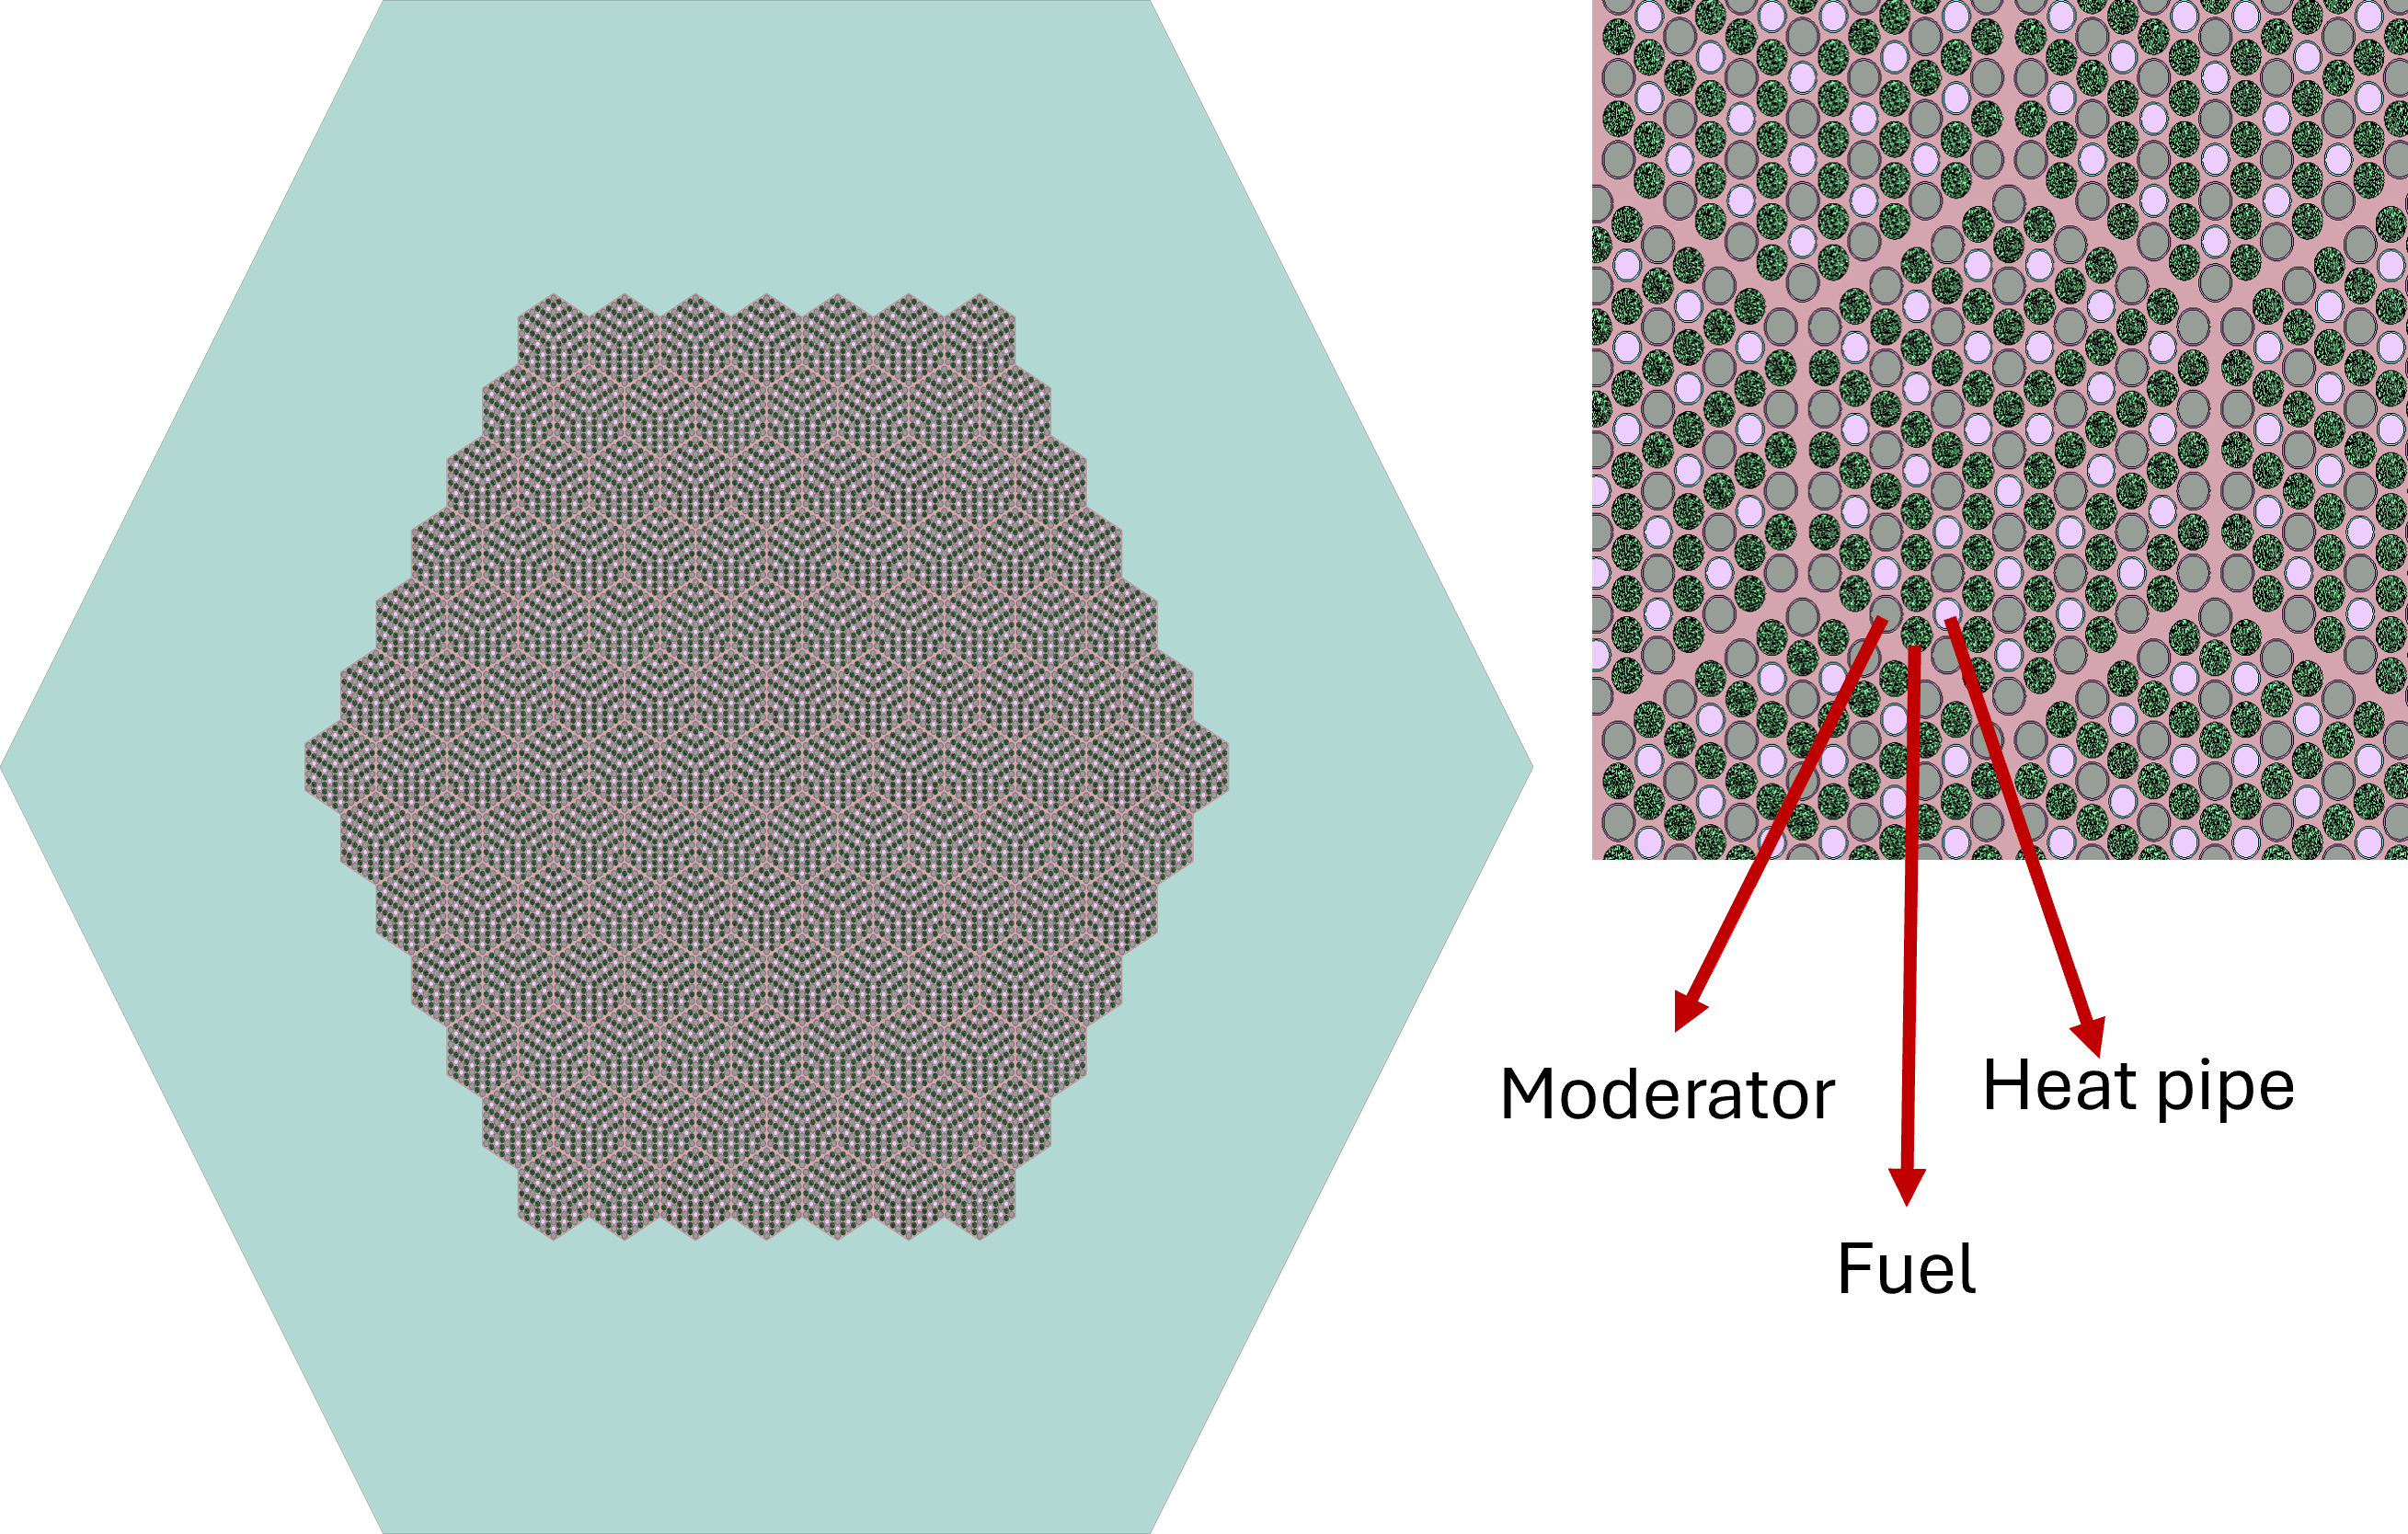
\includegraphics[width=120mm]{figures/VTB_core_and_assembly.png}
  \caption{System geometry.}
  \label{fig:VTB_geom}
\end{figure}



\section{Methodology}
\label{sec:methodology}

\subsection{The Fission Matrix Method}
\label{sec:fm_method}

The fission matrix (FM) method~\cite{CarneyANE2014} recasts the $k$-eigenvalue transport problem into a compact linear-algebraic form by partitioning the fissile domain into $N$ spatial regions and describing the transport between them over a single fission generation. Integrating the integral form of the $k$-eigenvalue transport equation over the volumes of a source region $j$ and a destination region $i$ yields
\begin{equation}
  S_i = \frac{1}{k}\sum_{j=1}^{N} a_{ij}\,S_j,
  \qquad\Longleftrightarrow\qquad
  \mathbf{A}\,\mathbf{S} = k\,\mathbf{S},
  \label{eqn:fm_eigen}
\end{equation}
where $S_j$ is the fission-neutron source integrated over region $j$, and the coefficient $a_{ij}$ is the expected number of fission neutrons born in region $i$ per fission neutron emitted in region $j$. The $N\times N$ array of these coefficients is the fission matrix $\mathbf{A}$: its dominant eigenvalue is $k_{\text{eff}}$ and the associated eigenvector is the regionwise fission-source distribution~\cite{CarneyANE2014}. 
% Throughout this work the column index $j$ labels the \emph{source} region and the row index $i$ the \emph{destination} region --- a convention that underlies the correlation structure derived in Sec.~\ref{sec:analytical_derivation}.

Because each coefficient is defined per emitted source neutron, the fission multiplicity is already embedded in it: a source neutron that induces a fission contributes $\bar\nu$ neutrons to the destination region, not one. The matrix is nonsymmetric, so its eigenvalues and eigenvectors are in general complex, although the fundamental mode is strictly real and non-negative~\cite{CarneyANE2014}. A key practical feature of the method is that the coefficients can be accumulated at negligible additional cost during an ordinary Monte Carlo criticality calculation, by tallying, over the active cycles, the region of birth of each fission neutron against the region of birth of its parent. In this work the full $127\times127$ fission matrix (one region per fuel assembly) is obtained in this way from a single whole-core Serpent calculation, so that every coefficient reflects the complete core environment.


\subsection{Database, Interpolation, and the Correction Ratio}
\label{sec:pipeline}

Rather than tallying a fission matrix directly for every temperature field of interest, the method precalculates a database of fission matrices at a set of uniform reference temperatures and interpolates within it. To keep the methodology practical and computationally attractive, it is important to maintain good accuracy while relying on a compact and simply defined database. For this reason, the database considered here contains the coefficients $a_{ij}$ at only eight uniform temperatures spanning 300--1000~K in 100~K increments. For an arbitrary temperature field, each coefficient is first obtained by piecewise-linear interpolation between the two bracketing database temperatures, as described in Eq.~\ref{eqn:interp}.

\begin{equation}
  a_{ij}(T_i) = a_{ij}^{-} + \frac{T_i - T_i^{-}}{T_i^{+} - T_i^{-}} \left( a_{ij}^{+} - a_{ij}^{-} \right),
  \label{eqn:interp}
\end{equation}

where $a_{ij}^{-}$ and $a_{ij}^{+}$ are the values of $a_{ij}$ at the database temperatures immediately below and above the arbitrary destination-cell temperature $T_i$.

Eq.~\ref{eqn:interp} treats each coefficient as depending only on the local temperatures "i", and therefore misses the influence of the surrounding temperature field. Under a large, spatially sharp gradient this is precisely where the interpolated matrix acquires a systematic error. The Core Temperature Correction Ratio (CTCR) defined in this work tries to compensate this by informing the numerical value of a generic matrix element $a_{ij}$, based on the couple of  temperatures $(T_i,T_j)$ trough a correction ratio $\hat r_{ij}$.
This correction is calibrated from two additional, directly simulated FMs, shown in Figure~\ref{fig:dirac_distributions} and described next.

\begin{figure}[h]
  \centering
  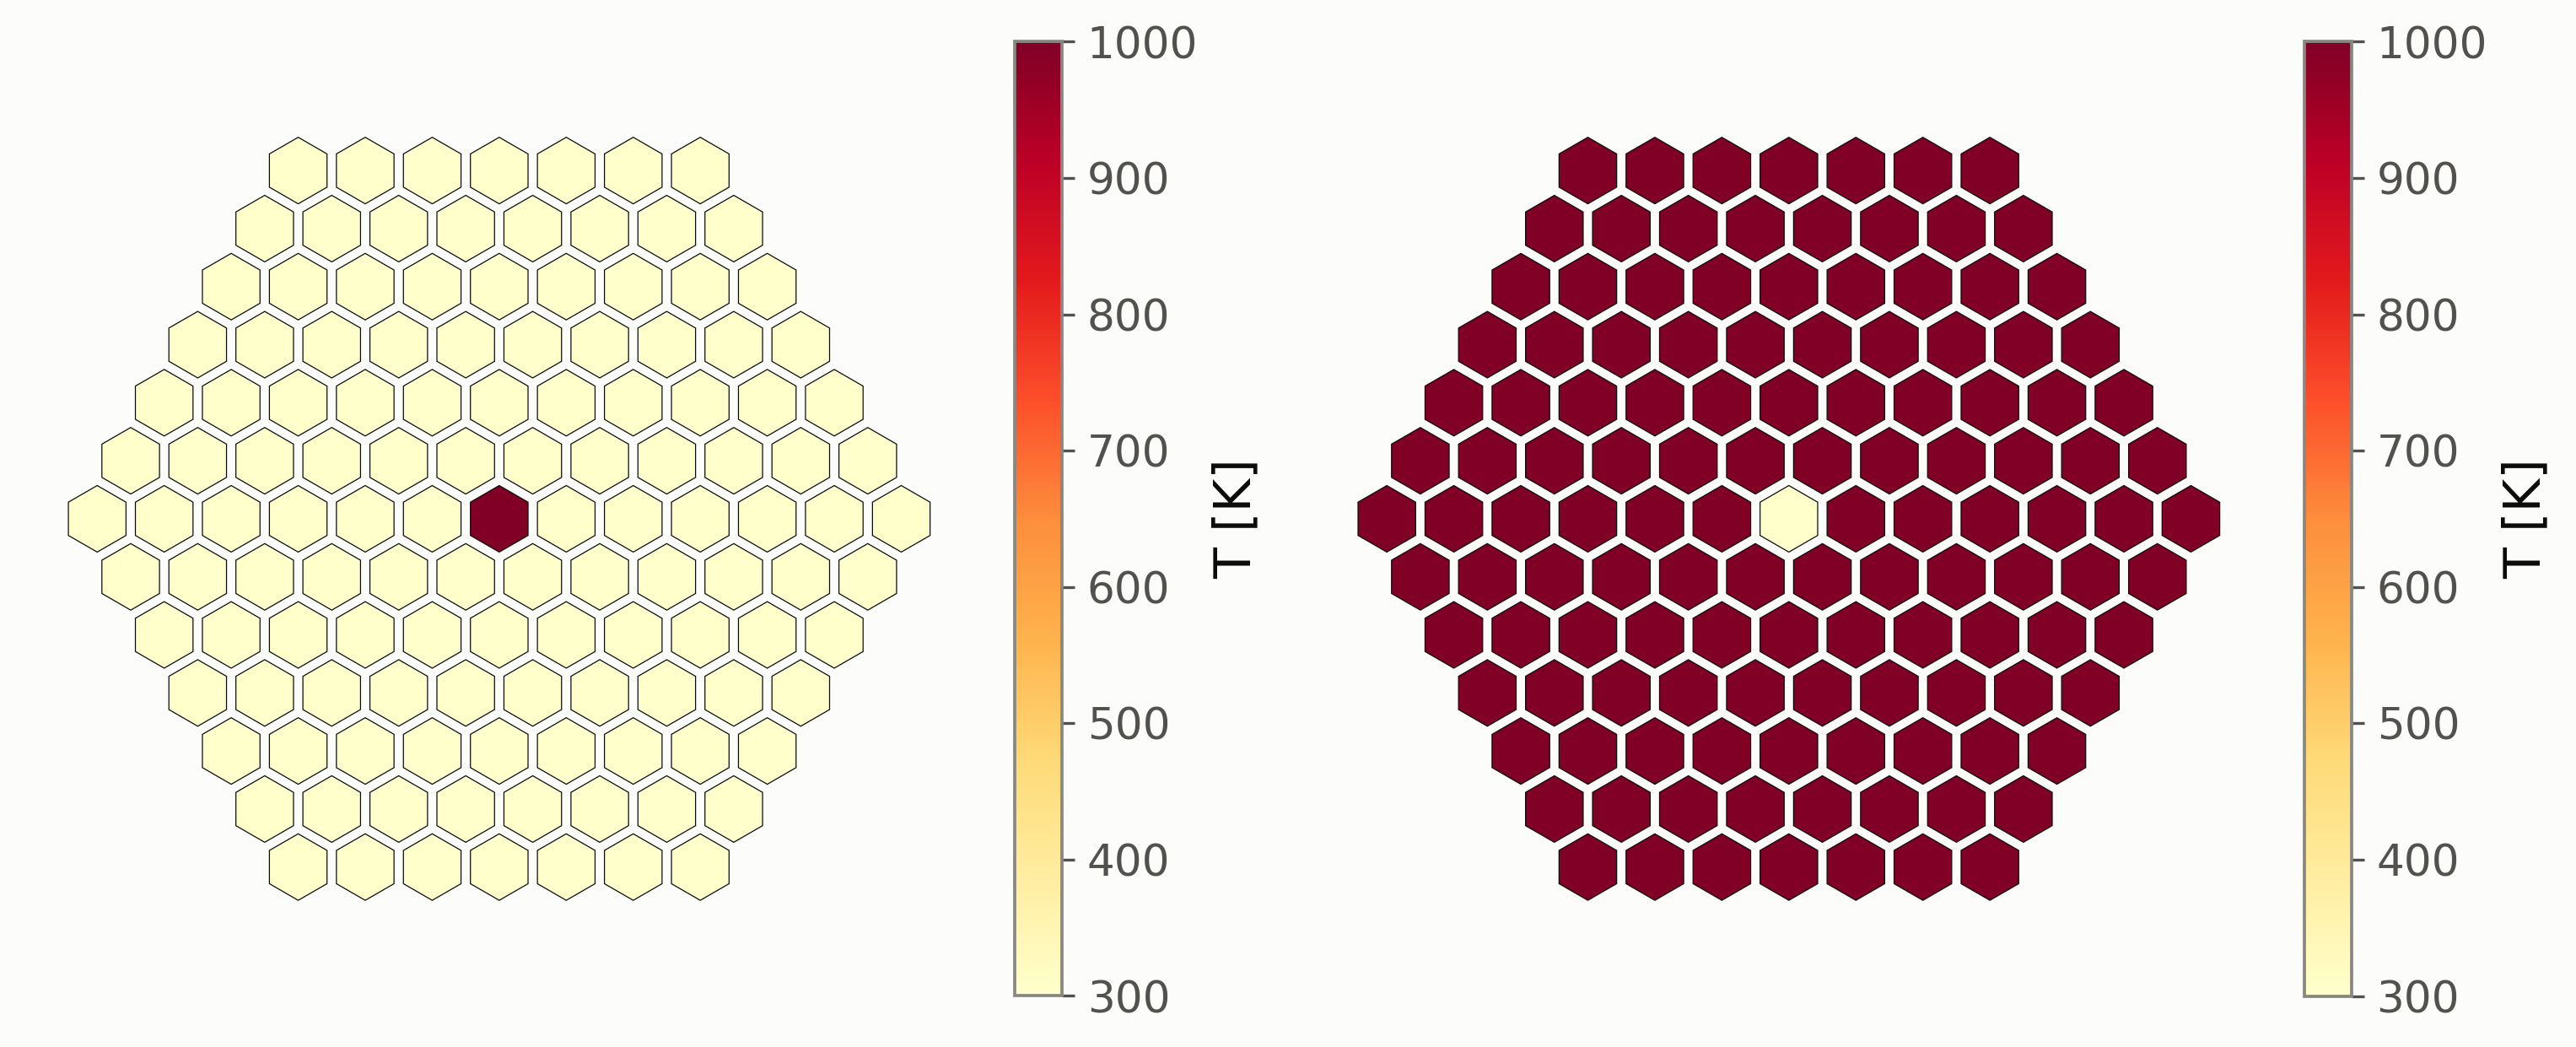
\includegraphics[width=140mm]{figures/fig_temp_dist_dirac1000.png}
  \caption{The "Dirac temperature distributions".}
  \label{fig:dirac_distributions}
\end{figure}


Because the correction must handle both a locally \emph{hot} cell embedded in a colder surrounding and the reverse case, both Dirac FMs of Figure~\ref{fig:dirac_distributions} are used: one with the central assembly $C$ driven to the hottest database temperature (1000~K) while the rest of the core sits at the coldest (300~K), and one with the assignment reversed. Comparing each Dirac FM against its own locally-interpolated counterpart gives two ratios, each a function of the geometric distance $d$ between $C$ and a generic cell $j$ (exploiting the hexagonal core's sextant symmetry, so that only $d$, not direction, matters),
\begin{equation}
  r^{+}(d) = \frac{a^{\text{dirac},+}_{Cj}}{a^{\text{interp}}_{Cj}},
  \qquad
  r^{-}(d) = \frac{a^{\text{dirac},-}_{Cj}}{a^{\text{interp}}_{Cj}},
  \label{eqn:ratio_def}
\end{equation}
where the superscript $+$ ($-$) denotes the hot-center (cold-center) Dirac case, and $a^{\text{interp}}_{Cj}$ is the coefficient the ordinary interpolation of Eq.~(\ref{eqn:interp}) would give for that same, uniform-elsewhere temperature field. Each ratio in isolation quantifies how much the local-temperature interpolation assumption misses, in the most extreme, most spatially sharp case the database can represent; combined, the two give the correction its ability to handle a temperature difference of either sign.

For an arbitrary temperature field, the correction applied to a generic interpolated coefficient $a^{\text{interp}}_{kl}$ is
\begin{equation}
  \hat r_{kl}(\Delta T_{kl}, d) = \frac{\Delta T_{kl}}{\Delta T_{\text{dirac}}} \left( r^{\pm}(d) - 1 \right) + 1,
  \qquad \Delta T_{kl} = T_k - T_l,
  \label{eqn:ctcr}
\end{equation}
where $\Delta T_{\text{dirac}} = 700$~K is the calibration temperature span common to both Dirac cases, and $r^{+}(d)$ is used when $\Delta T_{kl}>0$ (cell $k$ hotter than $l$) while $r^{-}(d)$ is used when $\Delta T_{kl}<0$ --- i.e., the calibration case matching the \emph{sign} of the local temperature difference, evaluated at its own geometric distance $d$.

In this work the two variants compared are referred to as \emph{raw} (interpolation only) and \emph{corrected} (interpolation plus CTCR).


\subsection{Two Sources of Uncertainty}
\label{sec:uncertainty}

Comparing an interpolated (and CTCR-corrected) result to a direct reference calculation involves two statistically independent Monte Carlo noise sources, which combine in quadrature:
\begin{equation}
  \sigma_{\text{tot}}^2 = \sigma_{\text{ref}}^2 + \sigma_{\text{interp}}^2 .
  \label{eqn:sigma_tot}
\end{equation}

\begin{itemize}
  \item[(a)] \emph{Reference-case noise}, $\sigma_{\text{ref}}$: the statistical uncertainty Serpent reports directly for the single reference simulation being compared against. 
  
  \item[(b)] \emph{Database noise}, $\sigma_{\text{interp}}$: the noise inherited by the interpolated (and corrected) matrix from the 8 database calculations it is built from. Unlike (a), this is not a quantity Serpent reports for any single run: the interpolated matrix is a new object with no MC replicas of its own, and must be constructed --- the subject of Sec.~\ref{sec:four_methods}.
\end{itemize}

\subsection{Quantification of $\sigma_{\text{interp}}$}
\label{sec:four_methods}

All four approaches proposed here share the same recipe: the nominal eight-temperature database is perturbed with random noise, the interpolator and correction of Eq.~(\ref{eqn:ctcr}) are reapplied, and the procedure is repeated many times. The spread of the resulting $k_{\text{eff}}^{\text{interp}}$ and fission source $F^{\text{interp}}$ over these repetitions is the database-side uncertainty $\sigma_{\text{database}}$.

What distinguishes the four approaches is how the random perturbation is generated. Writing the perturbation of the retained coefficients as a vector $\boldsymbol\delta$ drawn from a zero-mean multivariate normal distribution, $\boldsymbol\delta\sim\mathcal{N}(\mathbf{0},\boldsymbol\Sigma)$, the covariance $\boldsymbol\Sigma$ factors as
\begin{equation}
  \boldsymbol\Sigma = \mathbf{D}\,\boldsymbol\rho\,\mathbf{D},
  \label{eqn:sigma_factor}
\end{equation}
where $\mathbf{D}$ is the diagonal matrix of the per-coefficient standard deviations reported by Serpent, and $\boldsymbol\rho$ is the correlation matrix. The amplitude $\mathbf{D}$ is common to all approaches --- it is read directly from the nominal database --- so the four differ only in what they assume for $\boldsymbol\rho$: from neglecting correlation entirely, to predicting it analytically, to measuring it, to bypassing the construction altogether.

\begin{enumerate}
  \item[(i)] \textbf{Uncorrelated resampling ($\boldsymbol\rho=\mathbf{I}$).} Each retained coefficient is perturbed independently using only its own MC-reported variance, $a_{ij}\to a_{ij}+\delta_{ij}$ with $\delta_{ij}\sim\mathcal{N}(0,\sigma_{ij}^2)$. This is equivalent to setting $\boldsymbol\rho$ to the identity and is the simplified assumption adopted in prior FM uncertainty-quantification work~\cite{HeWaltersNSE2022}. It serves as the natural baseline against which to judge whether modeling correlation matters at all.

\item[(ii)] \textbf{Analytical model ($\boldsymbol\rho=\boldsymbol\rho_{\text{pred}}$).} The correlation matrix is predicted in closed form, $\boldsymbol\rho_{\text{pred}}$, derived in Sec.~\ref{sec:analytical_derivation} directly from the branching structure of the fission process. To the best of our knowledge, this closed-form prediction of the fission-matrix correlation structure from the branching process, and its use to build the interpolated matrix's uncertainty, has not been reported before: prior fission-matrix uncertainty-quantification work either neglects inter-coefficient correlation or estimates it empirically. The approach requires no Monte Carlo replicas beyond the single nominal database already needed for interpolation.

  \item[(iii)] \textbf{Correlated resampling, measured correlation ($\boldsymbol\rho=\hat{\boldsymbol\rho}$).} The correlation matrix is instead measured from the cycle-by-cycle tallies of a single MC run, treating each active cycle as a pseudo-replicate of the same underlying random vector. Since Serpent does not output the fission matrix on a per-cycle basis, this required a modification of the source code to tally and print each active cycle's fission matrix separately.
  % Because the number of cycles is smaller than the number of retained coefficients, the estimate is regularized with Ledoit--Wolf shrinkage.
  This $\hat{\boldsymbol\rho}$ is measured once, at 300~K, and reused unchanged at every other database temperature; the reasonableness of that reuse is examined in Sec.~\ref{sec:t_invariance}.

  \item[(iv)] \textbf{Brute force.} The full eight-temperature database is rebuilt from scratch $N=150$ times, with one genuinely independent MC replica per temperature per repetition, reapplying the interpolator and correction each time. This bypasses the $\boldsymbol\Sigma=\mathbf{D}\boldsymbol\rho\mathbf{D}$ construction entirely: correlations of every kind are present in the replicas by construction, with no modeling assumption. It is the most direct and most expensive estimate, and serves as the reference against which approaches (i)--(iii) are validated (Sec.~\ref{sec:validation}).
\end{enumerate}

% \subsection{Quantification of $\sigma_{interp}$}
% \label{sec:four_methods}

% In this work four different approaches are proposed to quantify $\sigma_{interp}$.
% All four approaches follow the same recipe: perturb the nominal 8-temperature database, refit the interpolator of Eq.~(\ref{eqn:ctcr}), and repeat many times. The spread of $k_{\text{eff}}^{\text{interp}}$ and the fission source $F^{\text{interp}}$ over those repetitions is $\sigma_{\text{database}}$.

% \begin{enumerate}
%   \item[(i)] \textbf{Uncorrelated resampling.} Each retained FM coefficient is perturbed independently, $a_{kl}\to a_{kl}+\delta_{kl}$, $\delta_{kl}\sim\mathcal{N}(0,\sigma_{kl}^2)$, using only its own MC-reported variance $\sigma_{kl}^2$. This is the simplified assumption used in prior FM uncertainty-quantification work~\cite{HeWaltersNSE2022}, and the natural baseline against which to judge whether modeling correlation matters at all.

%   \item[(ii)] \textbf{Analytical model.} $\boldsymbol\delta\sim\mathcal{N}(0,\boldsymbol\Sigma)$, $\boldsymbol\Sigma=\mathbf{D}\boldsymbol\rho_{\text{pred}}\mathbf{D}$, with $\rho_{\text{pred}}$ derived in Sec.~\ref{sec:analytical_derivation} from the branching structure of the fission process itself, requiring no MC replicas beyond the single nominal database already needed for interpolation.

%   \item[(iii)] \textbf{Correlated resampling, single-seed measured correlation.} $\boldsymbol\rho$ is instead measured directly from the cycle-by-cycle tallies of a single MC run (each active cycle treated as a pseudo-replicate of the same underlying random vector), regularized with Ledoit--Wolf shrinkage since the number of cycles is smaller than the number of retained coefficients. This $\boldsymbol\rho$ is estimated once, at 300~K, and reused unchanged at every other database temperature. We do not attempt a rigorous proof of temperature invariance here, only the simplest available check (Sec.~\ref{sec:t_invariance}): a $\boldsymbol\rho$ estimated independently at 1000~K is compared against the 300~K one, and against the internal noise floor of estimating $\boldsymbol\rho$ from half the data at a single, fixed temperature.

%   \item[(iv)] \textbf{Brute force.} The full 8-temperature database is rebuilt from scratch, independently, $N=150$ times --- one genuine, independent MC replica per temperature per repetition --- with the interpolator and CTCR reapplied each time. This is the most direct and most expensive estimate, used here as the reference against which (i)--(iii) are validated (Sec.~\ref{sec:validation}).
% \end{enumerate}

\subsection{Deriving the Analytical Correlation Model}
\label{sec:analytical_derivation}

Coefficients tallied within a single Monte Carlo criticality calculation are not, in general, statistically independent, because the number of neutron histories simulated per active cycle is fixed, a fact responsible for well-documented biases and correlations in cycle-based Monte Carlo estimators~\cite{BrissendenGarlick1986}. For two FM coefficients sharing the same source column $j$ (i.e., $a_{ij}$ and $a_{lj}$, $i\neq l$), this mechanism can be made concrete and, unlike the generic statement above, turned into a closed-form prediction.

At the start of a cycle, the number of source neutrons born in column $j$, $N_j$, is fixed (inherited from the previous cycle's fission bank). Each of these $N_j$ histories picks, independently of the others, exactly one outcome: it causes fission in some destination cell $i$ with probability $\pi_i$ (the same probability regardless of which of the $N_j$ histories is considered, since they are all born under identical conditions in column $j$), or it causes no fission at all, with the remaining probability. If it does cause fission, all $\bar\nu$ secondaries are born together at that one destination. Writing the contribution of history $s$ to destination $i$ as $X_s^{(i)} = \bar\nu\,I_s(i)$, where $I_s(i)$ is $1$ if history $s$ fissions in $i$ and $0$ otherwise, the retained coefficient is the per-source-neutron average
\begin{equation}
  a_{ij} = \frac{1}{N_j}\sum_{s=1}^{N_j} X_s^{(i)} .
  \label{eqn:aij_def}
\end{equation}

A single history cannot fission in two distinct destinations at once, so $I_s(i)\,I_s(l)=0$ for $i\neq l$, and different histories are independent of one another (linear transport: simulated particles do not interact). Hence, for a single history,
\begin{equation}
  \operatorname{Var}\left(X_s^{(i)}\right) = \bar\nu^2\,\pi_i(1-\pi_i), \qquad
  \operatorname{Cov}\left(X_s^{(i)},X_s^{(l)}\right) = \bar\nu^2\left[\underbrace{E\big(I_s(i)I_s(l)\big)}_{=\,0} - \pi_i\pi_l\right] = -\bar\nu^2\,\pi_i\pi_l ,
  \label{eqn:single_history}
\end{equation}
and summing $N_j$ independent, identically distributed histories (thus summing over $s$) and dividing by $N_j$ as in Eq.~(\ref{eqn:aij_def}),
\begin{equation}
  \operatorname{Var}(a_{ij}) = \frac{\bar\nu^2\,\pi_i(1-\pi_i)}{N_j}, \qquad
  \operatorname{Cov}(a_{ij},a_{lj}) = -\frac{\bar\nu^2\,\pi_i\pi_l}{N_j}, \qquad i\neq l .
  \label{eqn:multinomial_cov}
\end{equation}
The covariance is \emph{negative} for every pair of destinations sharing a source column, and this is not an approximation of the sign: it follows directly from the fact that a fixed number of histories are being split, exhaustively and mutually exclusively, among the possible destinations, so that more of $N_j$ going to $i$ mechanically means less going to $l$. Dividing the covariance by the geometric mean of the two variances, the common factor $\bar\nu^2/N_j$ cancels exactly, leaving a correlation that depends only on the destination probabilities themselves, not on $N_j$, which is a Serpent run-time setting, not a physical property of the fission process:
\begin{equation}
  \rho_{\text{pred}}(i,l) = \frac{\operatorname{Cov}(a_{ij},a_{lj})}{\sqrt{\operatorname{Var}(a_{ij})\operatorname{Var}(a_{lj})}}
  = -\sqrt{\frac{\pi_i}{1-\pi_i}\cdot\frac{\pi_l}{1-\pi_l}} .
  \label{eqn:rho_pi_form}
\end{equation}
Equation~(\ref{eqn:rho_pi_form}) is written in terms of the destination probabilities $\pi_i$, which are not directly tallied; what Serpent reports is the mean coefficient $a_i = \bar\nu\pi_i$ (the expected number of secondaries reaching $i$ per source neutron, i.e., $\pi_i = -\kappa a_i$ with $\kappa=-1/\bar\nu$). Substituting $\pi_i=-\kappa a_i$ into Eq.~(\ref{eqn:rho_pi_form}) and simplifying gives the closed form used for method (ii),
\begin{equation}
  \rho_{\text{pred}}(i,l) = \kappa\,\frac{\sqrt{a_i a_l}}{\sqrt{(1+\kappa a_i)(1+\kappa a_l)}}, \qquad \kappa=-\frac{1}{\bar\nu},
  \label{eqn:rho_pred}
\end{equation}
the closed form used for method (ii), requiring only $\bar\nu$ (from \texttt{NUBAR} in \texttt{\_res.m}) and the reference FM's own mean values --- no additional MC replicas. (The multinomial variance and covariance results used in Eqs.~(\ref{eqn:single_history})--(\ref{eqn:multinomial_cov}) are standard; see, e.g., Ref.~\cite{CasellaBerger2002}.)

\subsubsection{Why Coefficients in Different Columns Are Treated as Uncorrelated}
\label{sec:cross_column}

The argument above says nothing about coefficients that do \emph{not} share a column, $a_{ij}$ and $a_{kj'}$ with $j\neq j'$. It would be convenient, but not quite correct, to argue that $N_j$ and $N_{j'}$ are simply independent: the total population $N=\sum_j N_j$ is fixed by the simulation's particle count per cycle, so source regions compete for a shared budget and $\operatorname{Cov}(N_j,N_{j'})\neq0$ in general. This coupling, however, need not propagate to the \emph{normalized} coefficients themselves. By the law of total covariance,
\begin{equation}
  \operatorname{Cov}(a_{ij},a_{kj'}) = \underbrace{E\big[\operatorname{Cov}(a_{ij},a_{kj'}\mid N_j,N_{j'})\big]}_{\text{(I)}}
  + \underbrace{\operatorname{Cov}\big(E[a_{ij}\mid N_j],\, E[a_{kj'}\mid N_{j'}]\big)}_{\text{(II)}} .
  \label{eqn:total_cov_law}
\end{equation}
Term (I) vanishes because histories born in the disjoint columns $j$ and $j'$ are conditionally independent given $N_j,N_{j'}$ (again, no history-history interaction is assumed). Term (II) vanishes because $E[a_{ij}\mid N_j]=\pi_i$ is, by construction of the normalized estimator of Eq.~(\ref{eqn:aij_def}), a constant that does not depend on the realized value of $N_j$, so its covariance with anything is zero. This rules out one specific channel, competition for a shared per-cycle particle budget, as a source of cross-column correlation; it is not a claim that cross-column correlation is exactly zero for every other conceivable reason (e.g., spatially correlated local flux fluctuations, or the cycle-to-cycle propagation of the fission source itself~\cite{UekiNSE2003}), and a bootstrap check on 150 independent replicas at 300~K does find a small residual: coefficient pairs sharing a column are negative $59.95\%$ of the time (95\% CI $[59.48\%,60.30\%]$), against $51.13\%$ $[50.96\%,51.43\%]$ for pairs sharing a destination row and $51.20\%$ $[51.11\%,51.37\%]$ for pairs sharing neither --- both of the latter statistically distinguishable from the $50\%$ null, but by less than a tenth of the same-column effect. Method (ii) neglects this residual: a simplifying assumption, adopted because it is small relative to the effect being modeled, not a claim that it is absent. Its practical consequence is checked directly, not merely argued for, in Sec.~\ref{sec:validation}, where method (ii) is compared against a genuine brute-force reconstruction that makes no such assumption.

\subsubsection{Is Reusing One Correlation Matrix Across Temperature Reasonable?}
\label{sec:t_invariance}

Method (iii) assumes that the correlation matrix measured at 300~K also applies at the other database temperatures. The simplest test of this assumption is to measure $\boldsymbol\rho$ independently at the opposite end of the database range, 1000~K, and ask whether the two matrices differ by more than the statistical noise inherent in estimating either one.

Differences between correlation matrices are quantified here through the Frobenius norm, which treats an $N\times N$ matrix as a single vector of its entries and measures its Euclidean length,
\begin{equation}
  \|\mathbf{M}\|_F = \sqrt{\sum_{a=1}^{N}\sum_{b=1}^{N} M_{ab}^2}\,.
  \label{eqn:frobenius_norm}
\end{equation}
The distance between two matrices is the norm of their difference; normalizing by the norm of the reference matrix gives the dimensionless \emph{relative} Frobenius distance used throughout,
\begin{equation}
  d_F(\mathbf{A},\mathbf{B}) = \frac{\|\mathbf{A}-\mathbf{B}\|_F}{\|\mathbf{B}\|_F}\,,
  \label{eqn:frobenius_rel}
\end{equation}
so that $d_F=0$ for identical matrices and $d_F\!\sim\!1$ for matrices differing by an amount comparable to their own magnitude.

Table~\ref{tab:t_invariance} reports this distance between the 300~K and 1000~K matrices, alongside an internal noise floor for each temperature: the distance between two estimates of the \emph{same} matrix, obtained by splitting that temperature's own cycle data into two halves and measuring $\boldsymbol\rho$ from each. The noise floor is the distance one would obtain even if the true correlation matrix were exactly temperature-invariant, arising purely from the finite statistics of the estimate.

\begin{table}[h]
\centering
\caption{Simple Check of Temperature Invariance for the Measured Correlation Matrix}
\label{tab:t_invariance}
\begin{tabular}{lc}
\hline
Comparison & Relative Frobenius distance \\ \hline
$\boldsymbol\rho$(300~K) vs.\ $\boldsymbol\rho$(1000~K) & 0.643 \\
$\boldsymbol\rho$(300~K), split-half internal noise floor & 0.909 \\
$\boldsymbol\rho$(1000~K), split-half internal noise floor & 0.909 \\ \hline
\end{tabular}
\end{table}

The 300~K-vs-1000~K distance is \emph{smaller} than the noise floor of estimating $\boldsymbol\rho$ from half the data at a single, fixed temperature. By this measure the correlation matrix changes less between the two temperature extremes than a single-temperature estimate fluctuates under its own finite statistics, so reusing one matrix across the whole database is at least as reasonable as trusting the estimate at any one temperature on its own.


\subsection{Error Metrics}
\label{sec:metrics}

Two plain metrics are used throughout, deliberately without a covariance-weighted quadratic form such as a Mahalanobis distance: they are less sensitive to the \emph{spatial pattern} of a residual, but directly interpretable, which is what matters for the case-by-case comparison of Sec.~\ref{sec:results}. For $k_{\text{eff}}$,
\begin{equation}
  \Delta k_{\text{eff}} = k_{\text{eff}}^{\text{interp}} - k_{\text{eff}}^{\text{ref}}, \qquad
  z = \frac{\Delta k_{\text{eff}}}{\sigma_{\text{tot}}} ;
  \label{eqn:metrics_keff}
\end{equation}
For the fission source $F$ (normalized to unit sum over the 127 zones), the local relative deviation in each zone is defined as
\begin{equation}
  \delta F_i = \frac{F_i^{\text{interp}} - F_i^{\text{ref}}}{F_i^{\text{ref}}}\times 100\%,
  \label{eqn:metrics_fs_delta}
\end{equation}
and the overall discrepancy between the interpolated and reference source distributions is summarized by the root-mean-square (RMS) of the zone-wise relative deviations,
\begin{equation}
  \mathrm{RMS} = \sqrt{\left\langle \delta F_i^2 \right\rangle_i}.
  \label{eqn:metrics_fs}
\end{equation}
The RMS therefore provides a single scalar measure of the average relative error over the entire fission source distribution, without accounting for the spatial arrangement of the residuals.

Every uncertainty band reported in Sec.~\ref{sec:results} is $\pm2\sigma_{\text{tot}}$, matching the $|z|<2$ threshold used as the ``consistent with noise'' criterion, so that falling inside or outside a plotted band coincides with passing or failing that test. $\sigma_{\text{database}}$ in Eq.~(\ref{eqn:sigma_tot}) uses the analytical model (ii) throughout Sec.~\ref{sec:results}, validated next.


\section{Results}
\label{sec:results}

The pipeline is exercised on twelve validation cases, each a different in-core temperature field imposed on the HPMR model of Sec.~\ref{sec:geometry}, reported in Figure~\ref{fig:test_case_temperature_distribution_1} and Figure~\ref{fig:test_case_temperature_distribution_2}. They are chosen to span a wide range of spatial sharpness, since it is precisely under sharp gradients that the local-temperature interpolation assumption --- and hence the CTCR --- is most severely tested. The set comprises two spatially sharp ``Dirac'' perturbations, in which a single central assembly is offset in temperature from an otherwise uniform core; a six-assembly and two ring-shaped hot-spot patterns; a smooth linear gradient across the core; and six power-shaped profiles of varying peak sharpness and radial offset. Each case is evaluated in both the \emph{raw} (interpolation only) and \emph{corrected} (interpolation plus CTCR) variants of Sec.~\ref{sec:pipeline}, against a direct Serpent reference calculation of the same temperature field.

\begin{figure}[t]
  \centering
  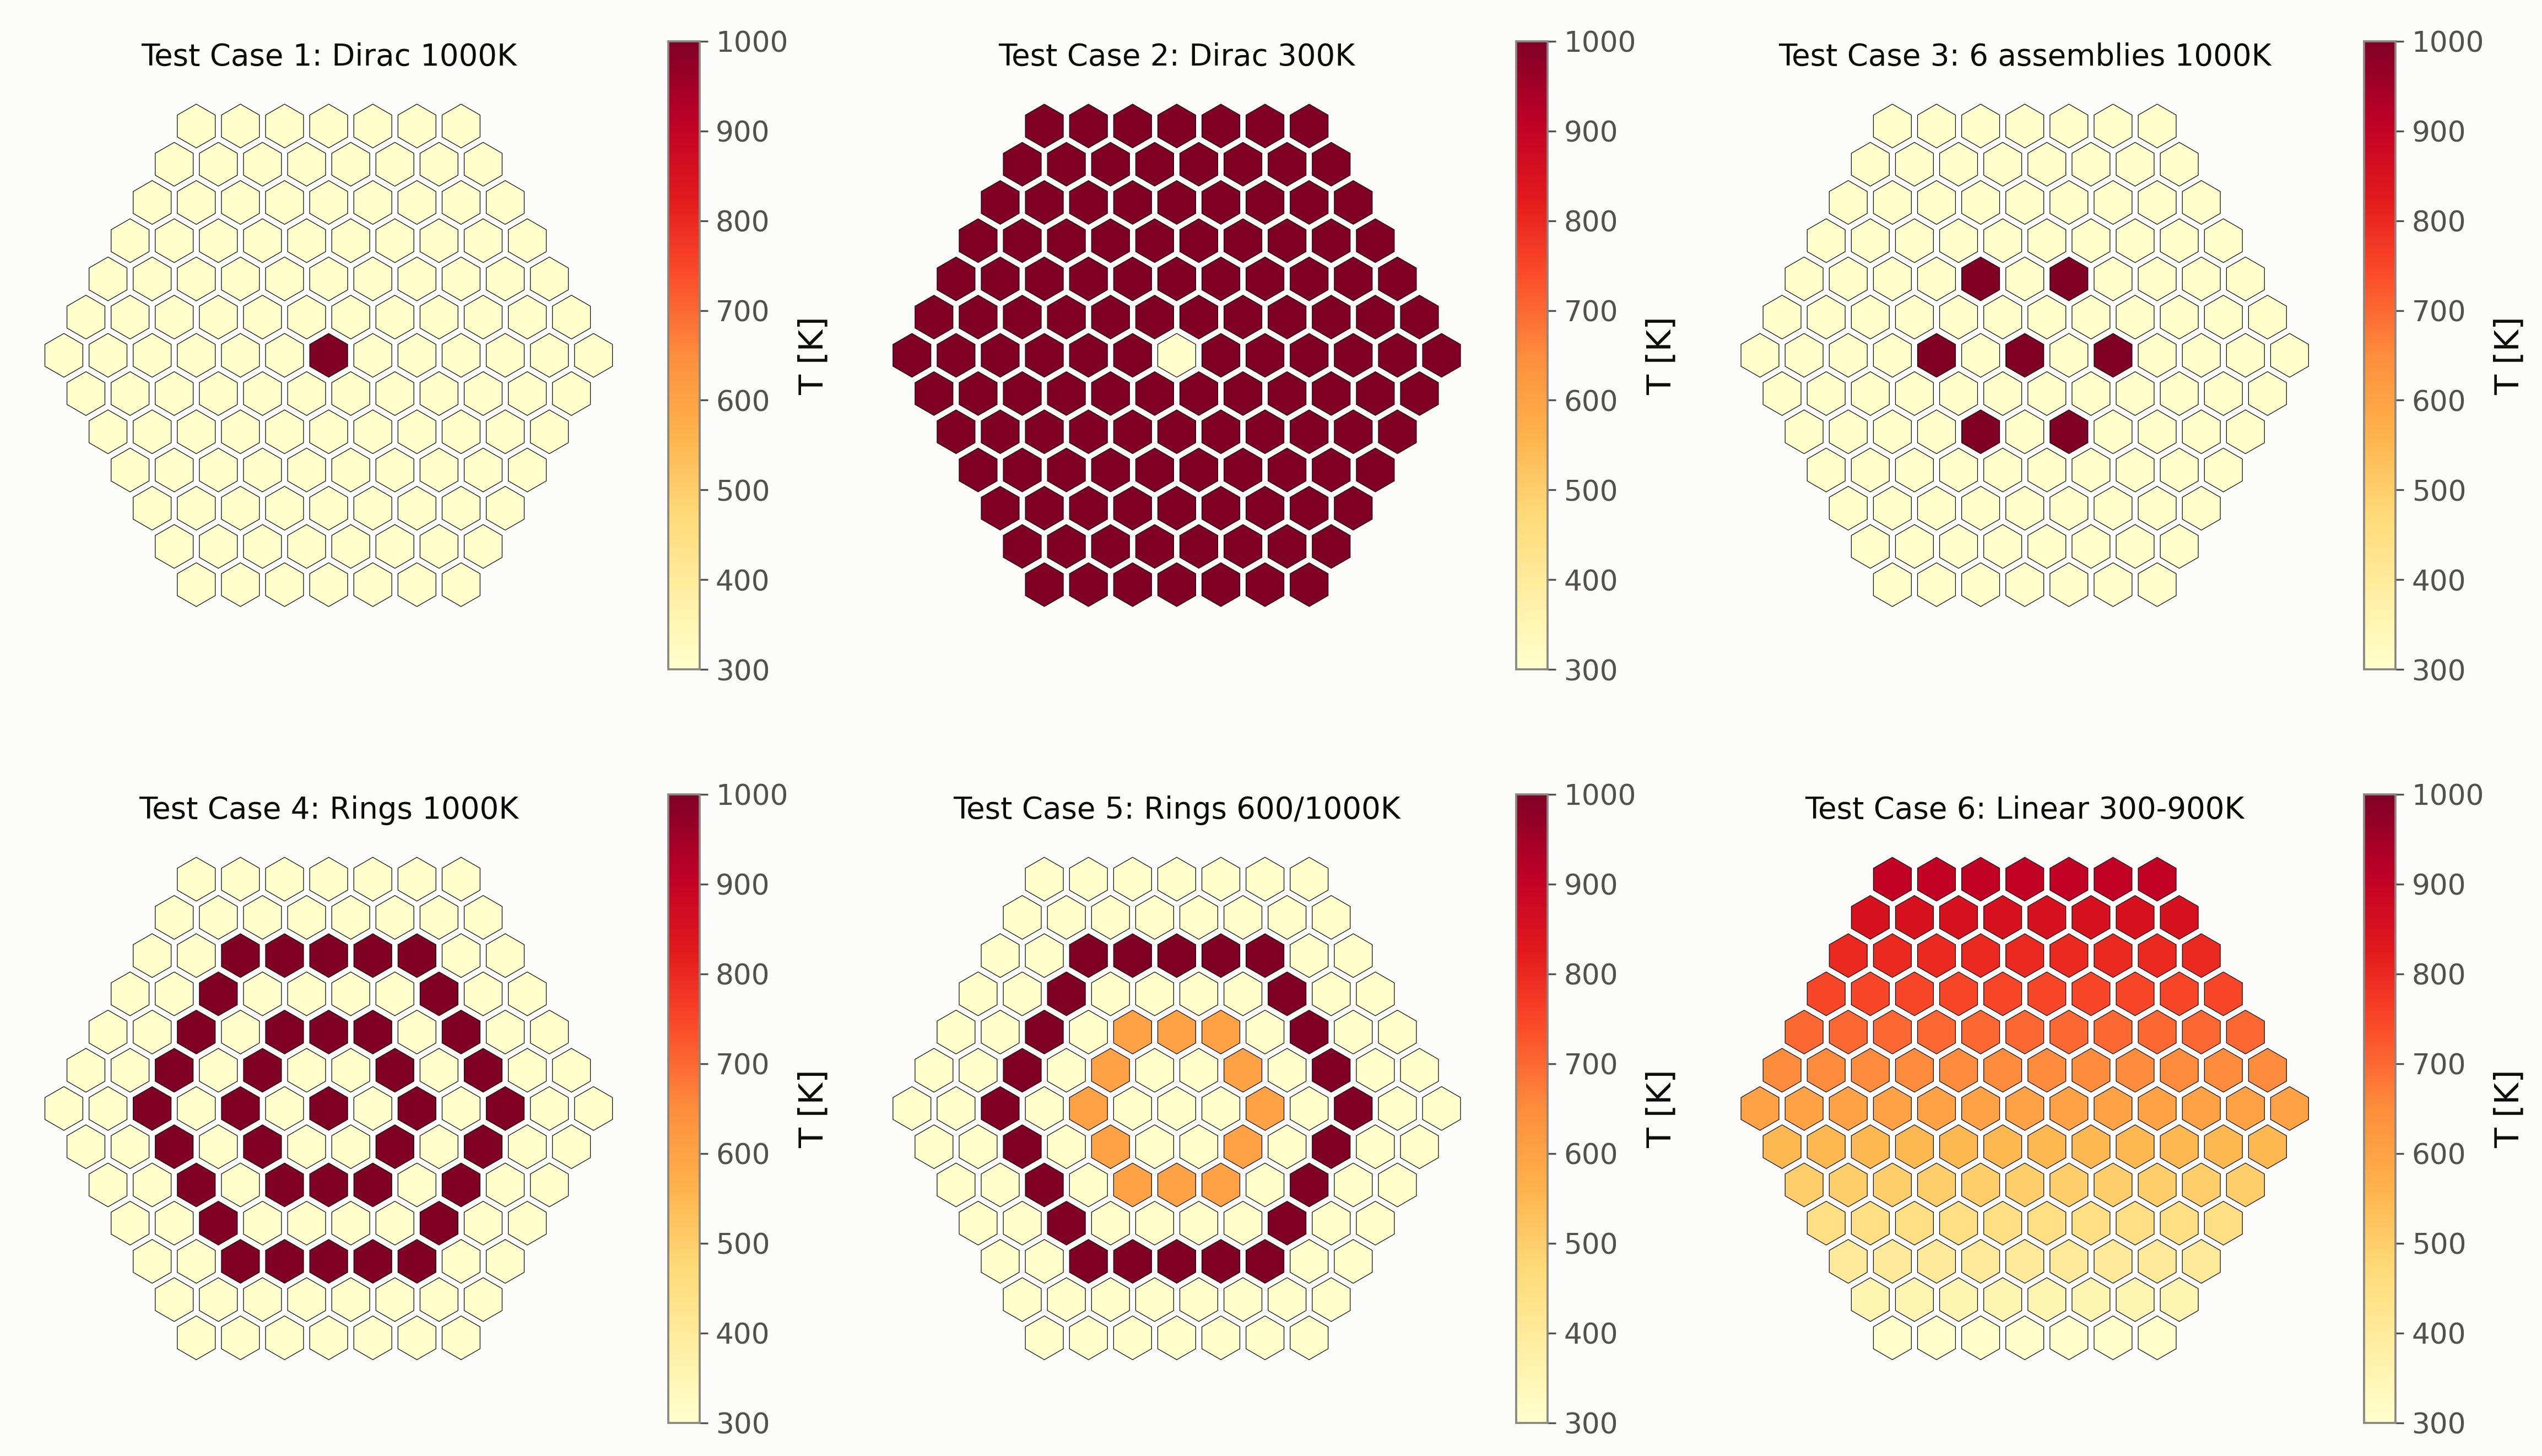
\includegraphics[width=160mm]{figures/fig5a_temperature_distributions.png}
  \caption{Reference-cases temperature distribution.}
  \label{fig:test_case_temperature_distribution_1}
\end{figure}

\begin{figure}[t]
  \centering
  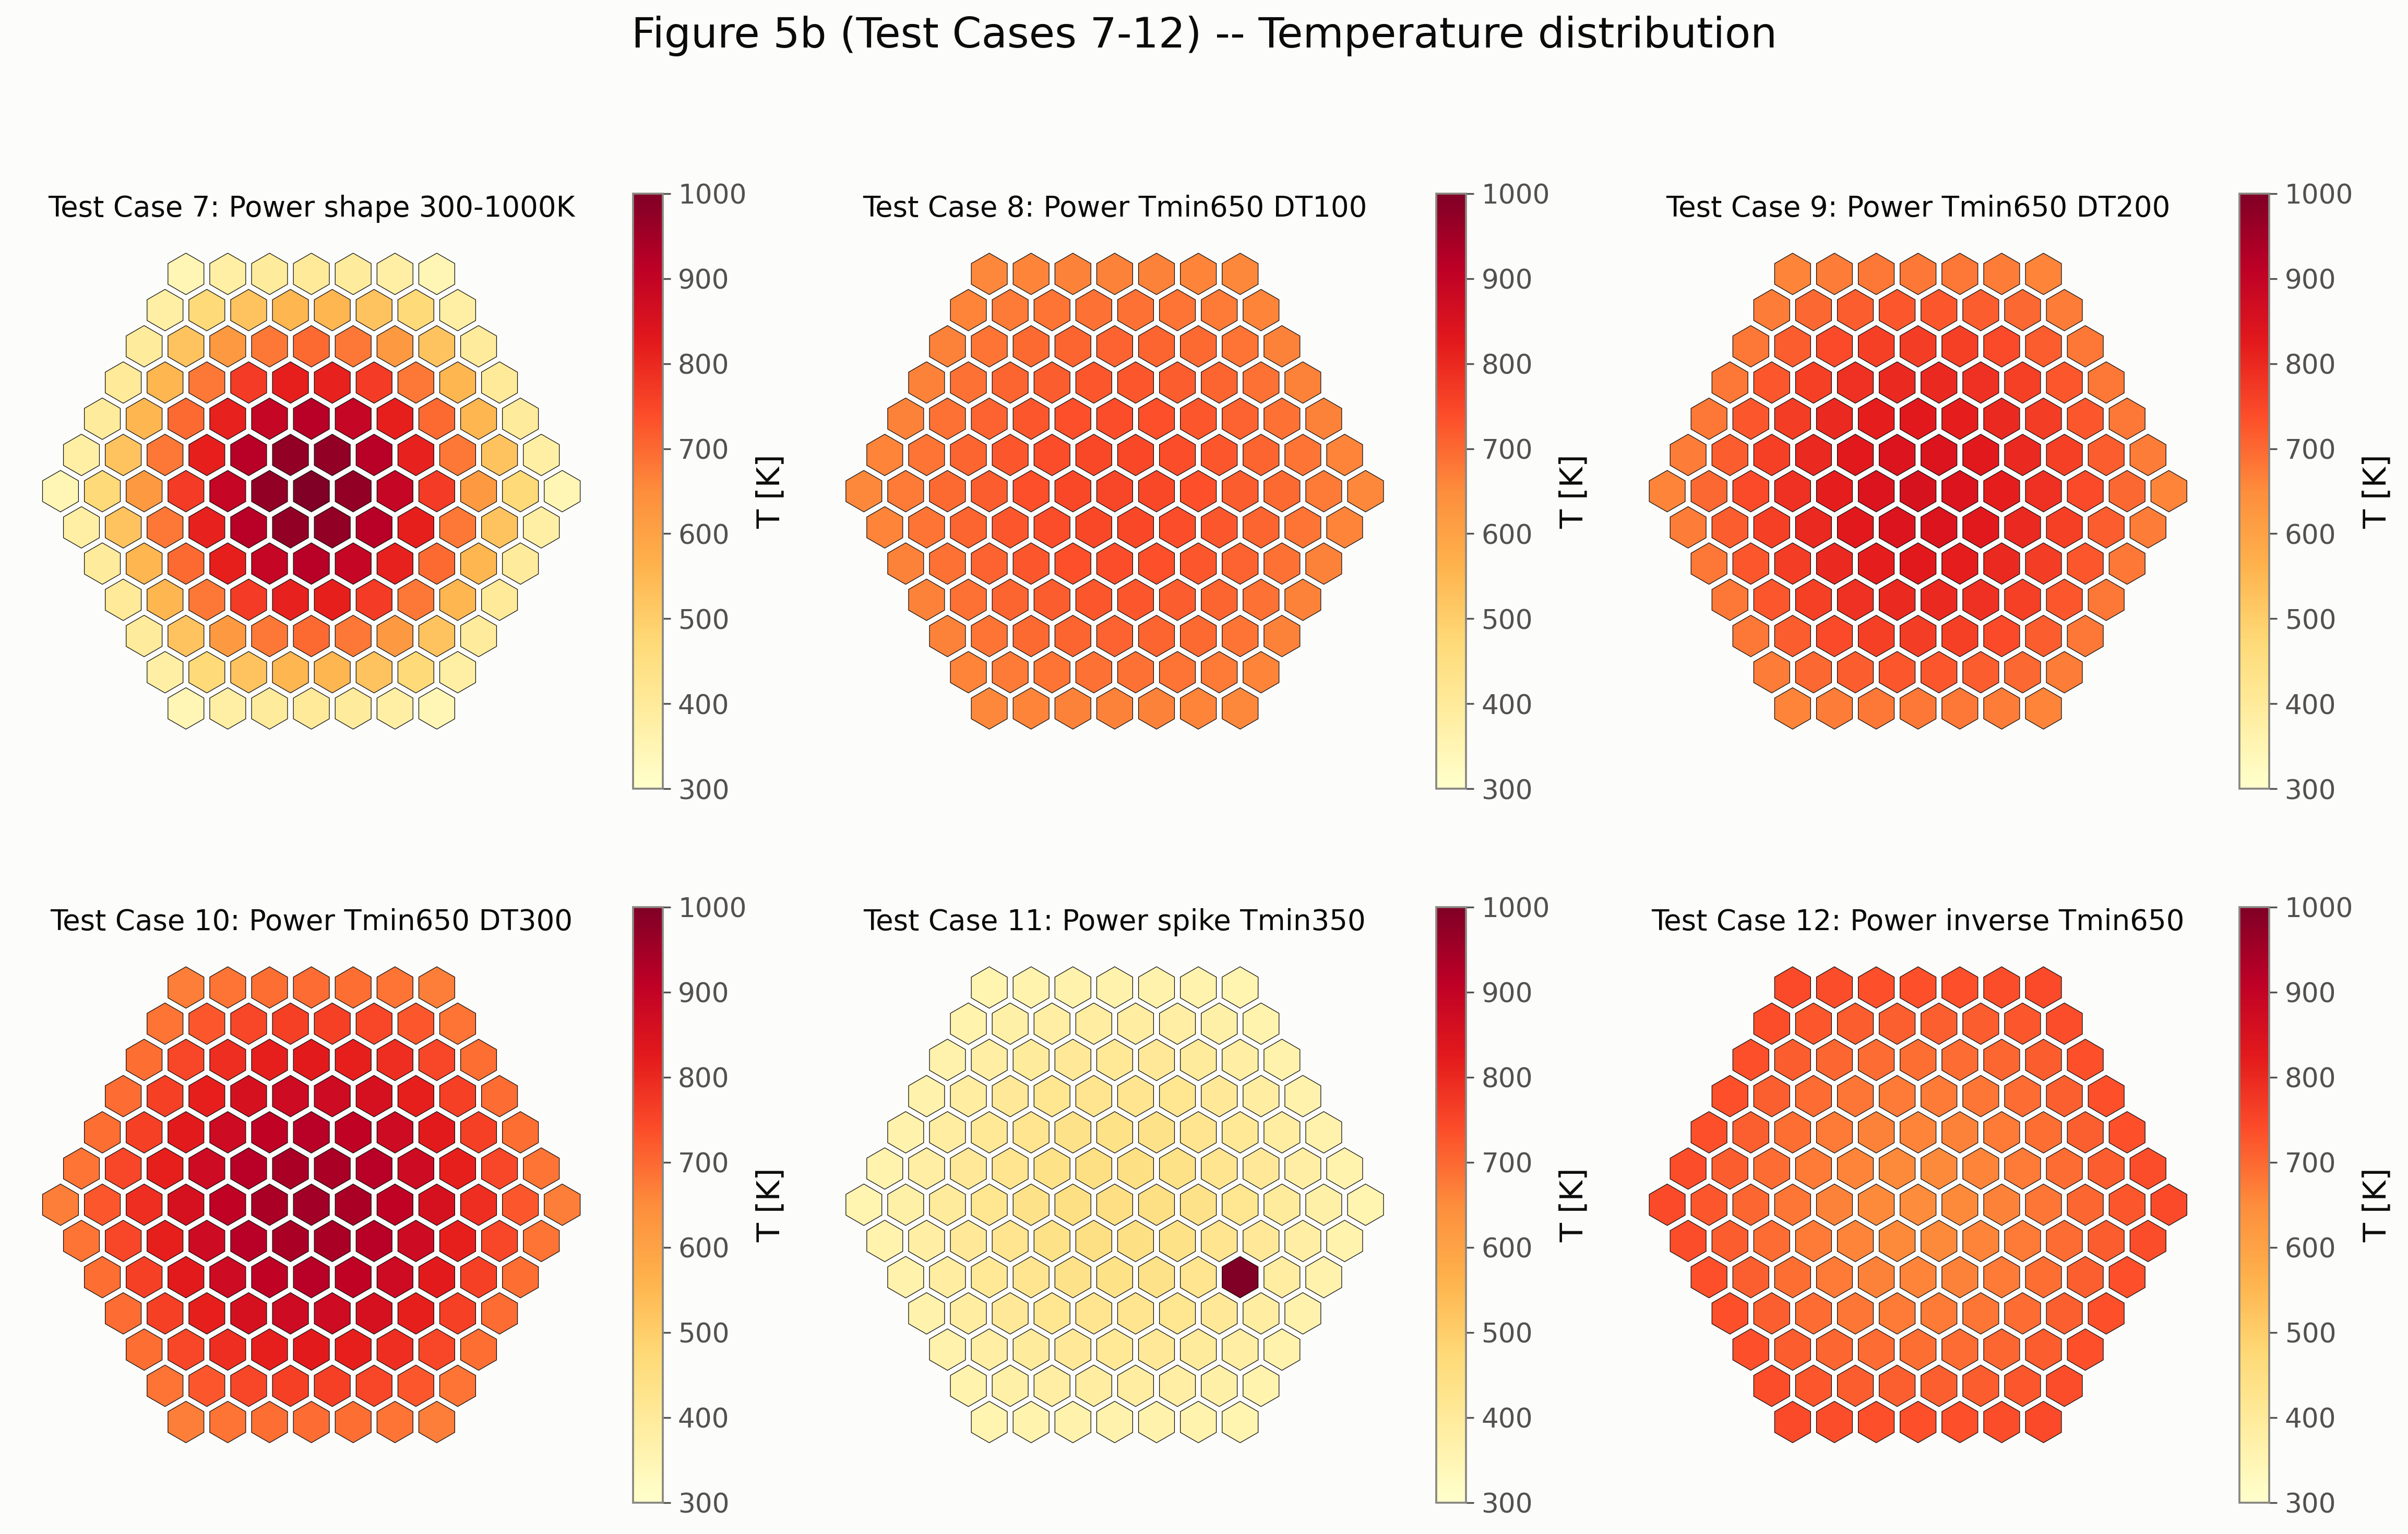
\includegraphics[width=160mm]{figures/fig5b_temperature_distributions.png}
  \caption{Reference-cases temperature distribution.}
  \label{fig:test_case_temperature_distribution_2}
\end{figure}


\subsection{Reference-Case Uncertainty}
\label{sec:res_reference}

Figure~\ref{fig:fig1} shows the reference-case uncertainty $\sigma_{\text{ref}}$, source (a) of Sec.~\ref{sec:uncertainty}, on its own. Averaged over the twelve cases it is 9.7~pcm on $k_{\text{eff}}$ and 0.309\% (RMS) on the fission source, and is essentially uniform across cases; the one mild outlier is the Power shape 300--1000~K case (12.5~pcm, 0.42\%), whose broader, shallower temperature profile produces a less peaked fission-source distribution and hence a statistically noisier detector tally. This is only half of the noise budget of Eq.~(\ref{eqn:sigma_tot}): on its own it says nothing about the uncertainty introduced by the interpolation, quantified next.

\begin{figure}[t]
  \centering
  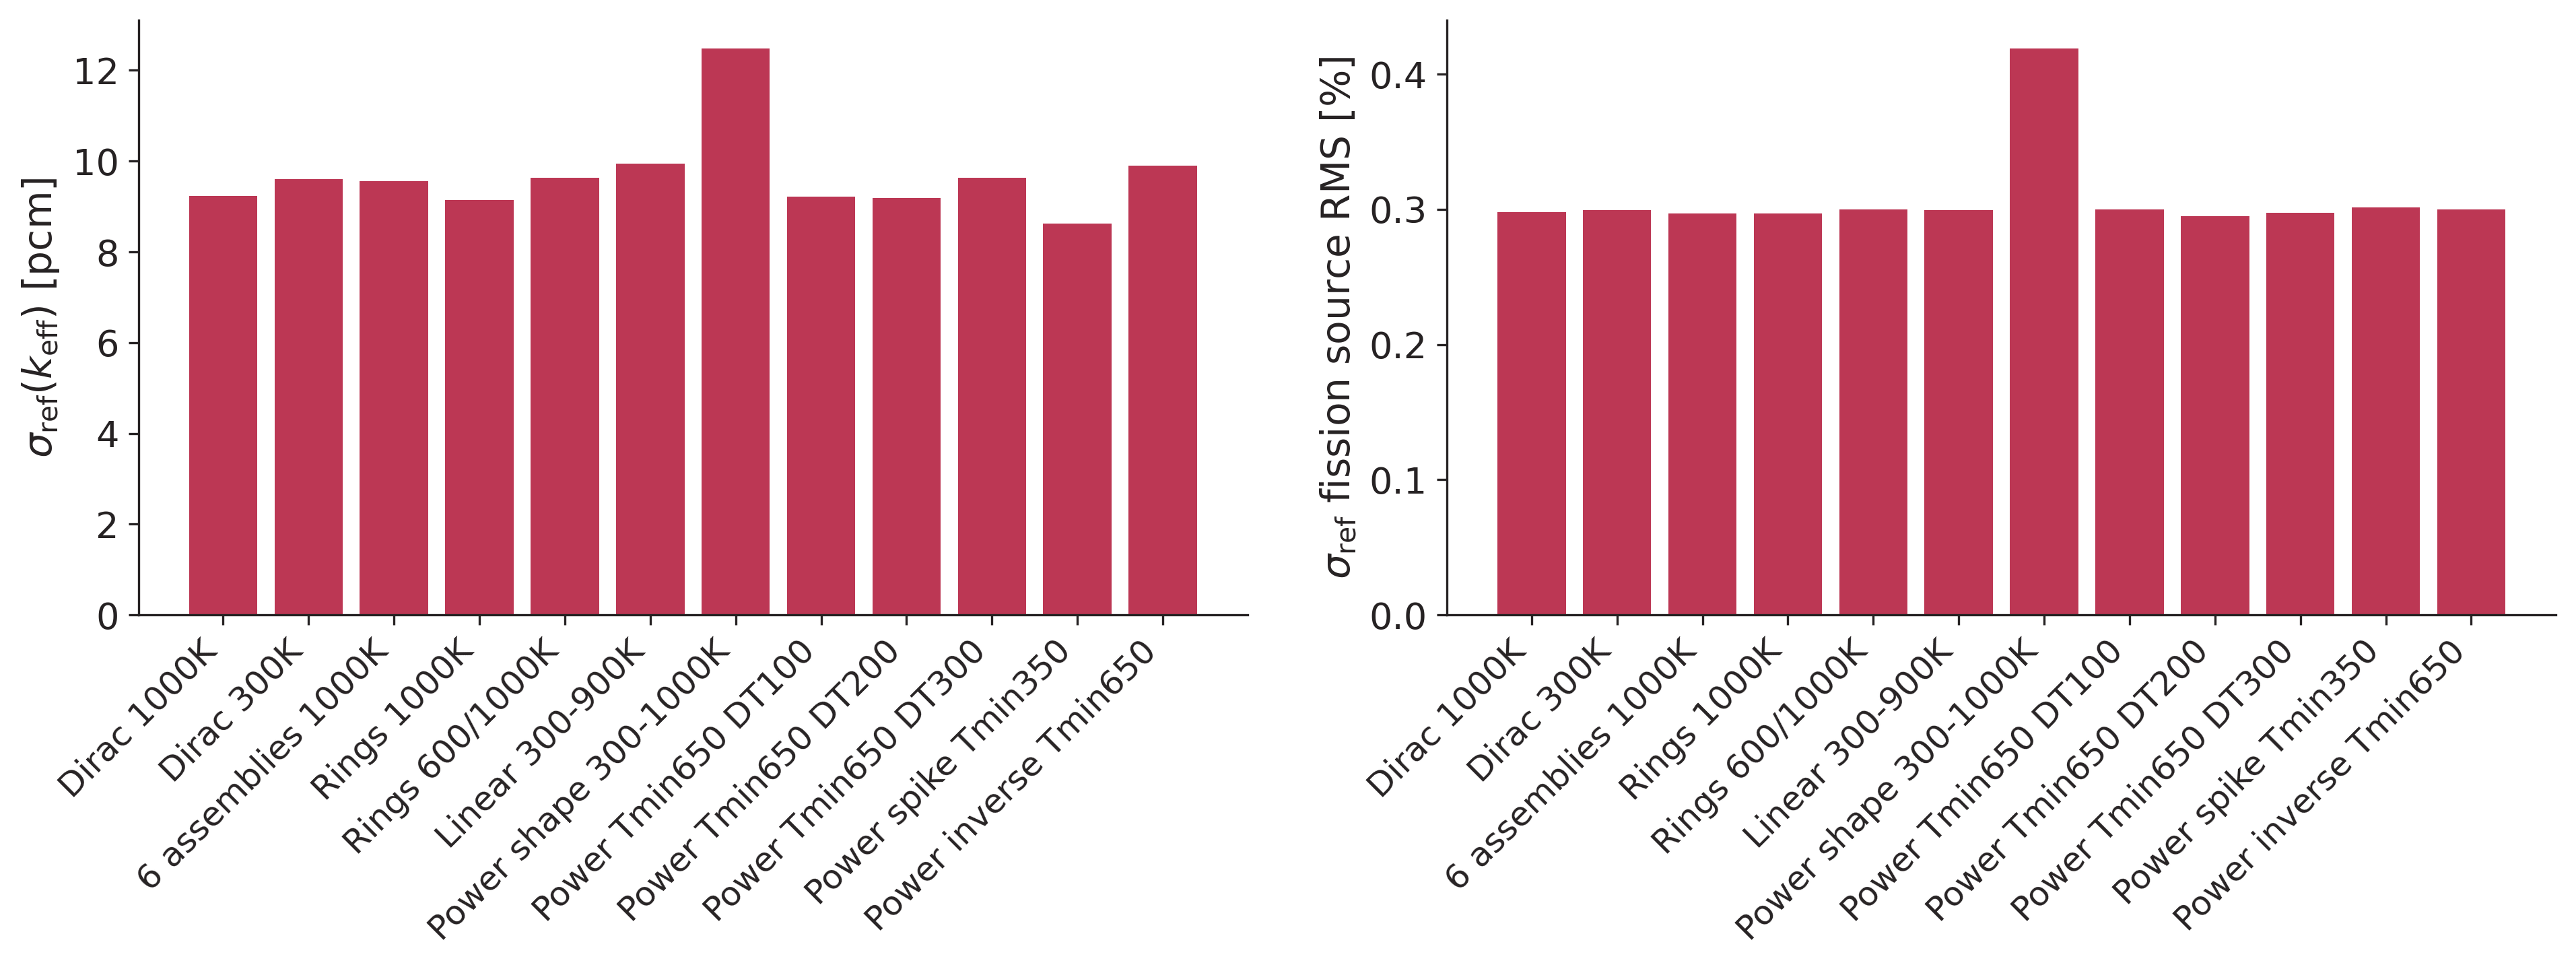
\includegraphics[width=140mm]{figures/fig1_reference_case_uncertainty.png}
  \caption{Reference-case Monte Carlo uncertainty $\sigma_{\text{ref}}$: $k_{\text{eff}}$ (left, from \texttt{\_res.m}) and fission-source RMS (right, from \texttt{\_det0.m}), for all twelve cases.}
  \label{fig:fig1}
\end{figure}

\subsection{Validating the Database-Noise Models Against Brute Force}
\label{sec:validation}

Figure~\ref{fig:fig2} compares the three inexpensive approaches of Sec.~\ref{sec:four_methods}, uncorrelated (i), analytical (ii), and single-seed measured (iii),against the brute-force reconstruction (iv), for the corrected variant of all twelve cases, on both observables. Agreement is summarized by the mean absolute deviation from brute force across the twelve cases.
The ordering of the interpolated uncertainties $\sigma_{\text{interp}}$ predicted by the three models, excluding the brute-force results, which are used here as reference, is consistent with expectations in almost all the test cases. The uncorrelated model
systematically yields the largest $\sigma_{\text{interp}}$, and therefore the widest
confidence intervals, the only exception being $k_{\text{eff}}$ in Test Case~4; the
analytical covariance model gives the smallest values, while the measured covariance
matrix lies in between. This single exception can be ascribed to statistical noise: the
database is resampled randomly from a Gaussian distribution centered on the nominal
values, so fluctuations of this magnitude are not unexpected. 

\begin{figure}[h]
  \centering
  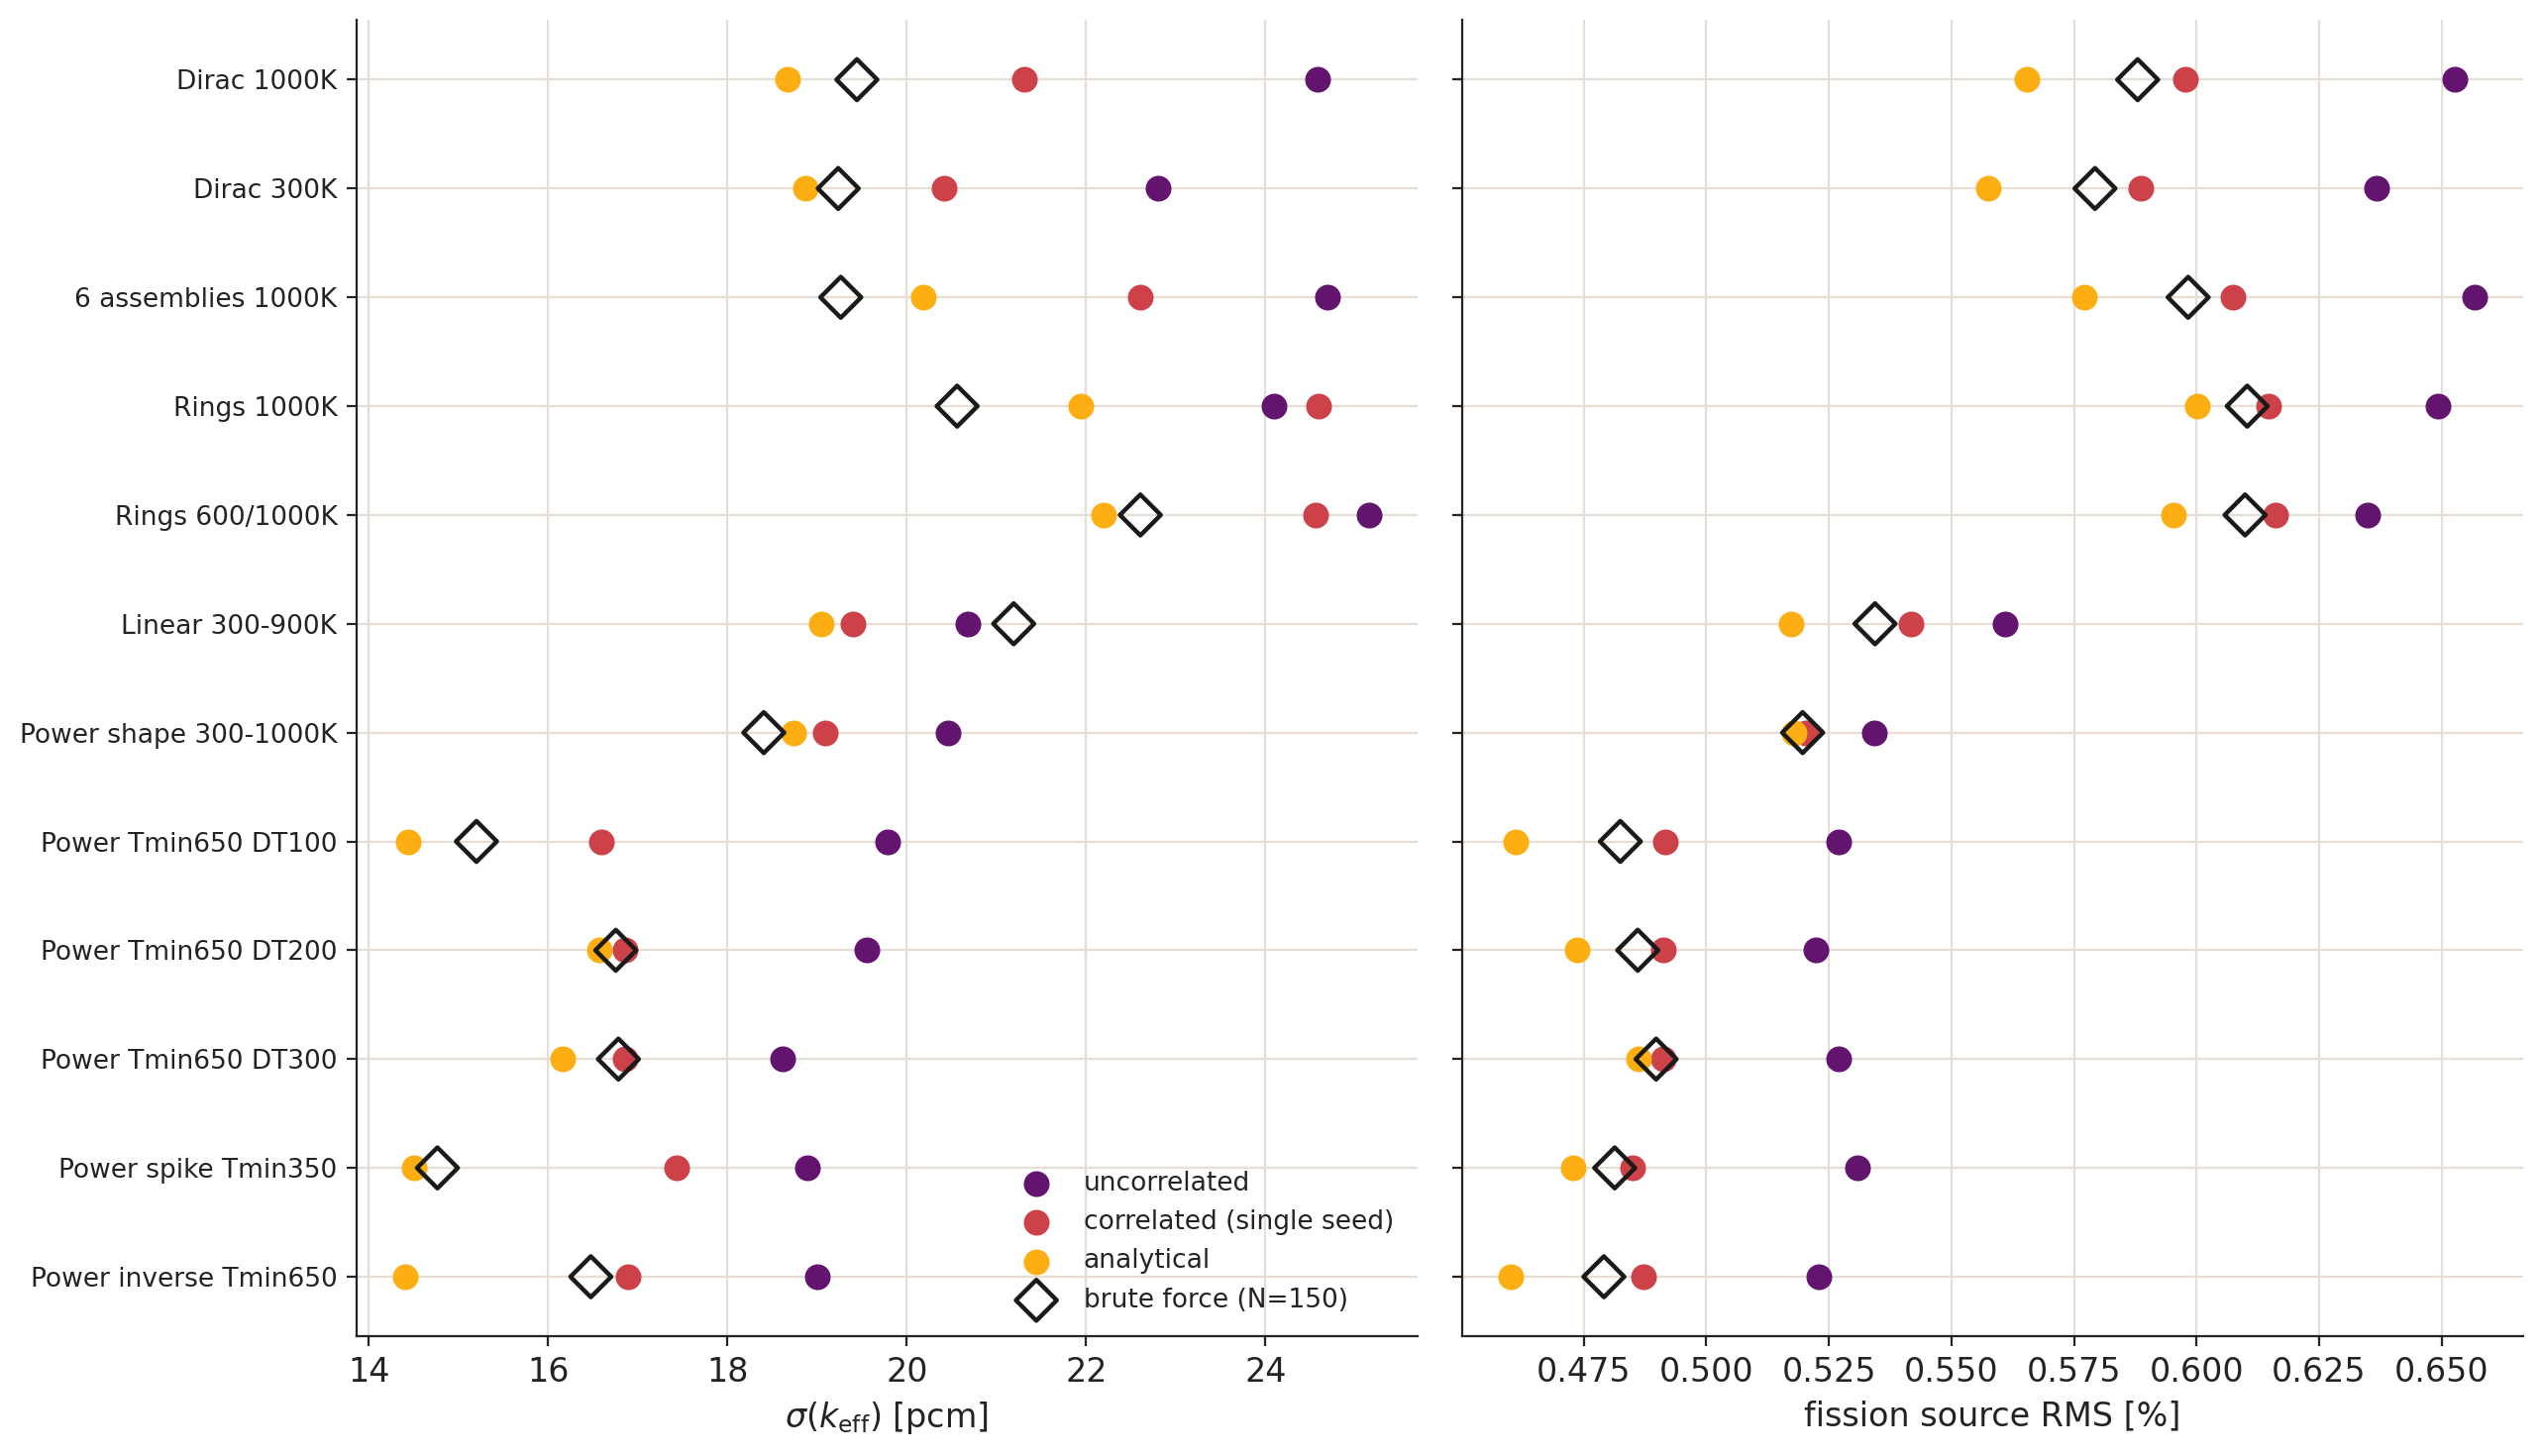
\includegraphics[width=140mm]{figures/fig2_validation_against_brute_force (1).png}
  \caption{Database-side uncertainty predicted by methods (i)--(iii) of Sec.~\ref{sec:four_methods} against the brute-force reference (iv, $N=150$): $k_{\text{eff}}$ (left) and fission-source RMS (right), corrected variant, all twelve cases.}
  \label{fig:fig2}
\end{figure}


On $k_{\text{eff}}$, the analytical model is the closest of the three, reproducing the brute-force uncertainty to within 4.6\%, ahead of the single-seed measured model (8.7\%) and well ahead of the uncorrelated model (18.0\%). The ordering confirms what the derivation of Sec.~\ref{sec:analytical_derivation} predicts: the intra-column correlations are negative, so neglecting them (method i) inflates the propagated $k_{\text{eff}}$ variance, while capturing them in closed form (method ii) does not require the additional simulation that measuring them (method iii) does. On the fission-source RMS the ranking changes: the single-seed (3.3\%) and the analytic (3.6\%) models track brute force more closely than the uncorrelated one (7.3\%). This is consistent with the cross-column residual left unmodeled by method (ii) (Sec.~\ref{sec:cross_column}): the fission source is a less global quantity, sensitive to correlations between coefficients in different columns in a way the eigenvalue is not, so the very terms the analytical model omits matter more here.

Despite not being uniformly best, the analytical model is adopted for both observables in the combined uncertainty value of Sec.~\ref{sec:res_final}: on both it remains within the same order of magnitude as the brute-force reference, and it alone requires no Monte Carlo replicas beyond the nominal database: the practical criterion this work is built around.



% \subsubsection{Stability of the Analytical Model}
% \label{sec:stability_of_analytic_model}

% One could object that the analytical model is not truly independent of Monte Carlo noise: the closed form of Eq.~(\ref{eqn:rho_pred}) is evaluated on the mean coefficients $a_i$ of a single database, which are themselves affected by statistical uncertainty. Had a different random seed been used, the predicted matrix $\boldsymbol\rho_{\text{pred}}$ would differ slightly, and one may ask whether that sensitivity matters.

% To test this, $\boldsymbol\rho_{\text{pred}}$ at 300~K was rebuilt from each of the 150 independent seeds of the brute-force set and compared, through the relative Frobenius distance of Eq.~(\ref{eqn:frobenius_rel}), against the matrix built from the production seed. The seed-to-seed spread is negligible: a mean distance of 0.0013 and a maximum of 0.0014, two to three orders of magnitude below both the temperature dependence of the measured matrix (0.643) and its single-temperature noise floor (0.909, Sec.~\ref{sec:t_invariance}). The Monte Carlo noise in the mean FM coefficients is therefore not a meaningful source of uncertainty for the analytical model, and $\boldsymbol\rho_{\text{pred}}$ can be treated as effectively deterministic.

\subsubsection{Stability of the Analytical Model}
\label{sec:stability_of_analytic_model}

One could object that the analytical model is not truly independent of Monte Carlo noise: the closed form of Eq.~(\ref{eqn:rho_pred}) is evaluated on the mean coefficients $a_i$ of a single database, which are themselves affected by statistical uncertainty. Had a different random seed been used, the predicted matrix $\boldsymbol\rho_{\text{pred}}$ would differ slightly, and one may ask whether that sensitivity matters.

To test this, $\boldsymbol\rho_{\text{pred}}$ at 300~K was rebuilt from each of the 150 independent seeds of the brute-force set and compared, through the relative Frobenius distance of Eq.~(\ref{eqn:frobenius_rel}), against the matrix built from the production seed (Table~\ref{tab:rho_pred_stability}).

\begin{table}[h]
\centering
\caption{Sensitivity of $\boldsymbol\rho_{\text{pred}}$ to the Database Seed (300~K)}
\label{tab:rho_pred_stability}
\begin{tabular}{lc}
\hline
Seed-to-seed spread & Relative Frobenius distance \\ \hline
Mean & 0.0013 \\
{}[16, 84] percentile & $[0.0013,\ 0.0013]$ \\
Maximum & 0.0014 \\ \hline
\end{tabular}
\end{table}

The seed-to-seed spread is negligible: two to three orders of magnitude below both the temperature dependence of the measured matrix (0.643) and its single-temperature noise floor (0.909, Sec.~\ref{sec:t_invariance}). The Monte Carlo noise in the mean FM coefficients is therefore not a meaningful source of uncertainty for the analytical model, and $\boldsymbol\rho_{\text{pred}}$ can be treated as effectively deterministic.


\subsection{Does the Correction Ratio Help at the Point-Estimate Level?}
\label{sec:res_raw_vs_corrected}

Figure~\ref{fig:fig3} compares raw and corrected interpolation against the direct reference, before any uncertainty is folded in, and Table~\ref{tab:reference_results} reports the underlying per-case numbers. Averaged over the twelve cases, the CTCR reduces the mean absolute $k_{\text{eff}}$ discrepancy from 40.8 to 31.0~pcm (24\%) and the mean fission-source RMS discrepancy from 1.27\% to 0.96\% (25\%). The benefit is markedly uneven. It is largest for the sharpest, most localized profiles --- Rings 1000~K improves from $57.4$ to $0.7$~pcm, and 6~assemblies 1000~K from $53.9$ to $23.5$~pcm --- consistent with the CTCR having been calibrated against a sharp central perturbation. For smoother, less localized profiles it is negligible or mildly unfavorable, the Power Tmin650 DT200 case worsening from $-41.5$ to $-52.5$~pcm. This geometric dependence is expected from the way the correction is constructed (Sec.~\ref{sec:pipeline}): calibrated on a Dirac-like perturbation, it is most effective where the true field most resembles one.

\begin{table}[h]
\centering
\caption{Point-Estimate Discrepancy Against the Direct Reference, All Twelve Cases}
\label{tab:reference_results}
\begin{tabular}{lcccc}
\hline
 & \multicolumn{2}{c}{$\Delta k_{\text{eff}}$ [pcm]} & \multicolumn{2}{c}{Fission-source RMS [\%]} \\
Case & raw & corrected & raw & corrected \\ \hline
Dirac 1000~K            & 79.7  & 13.5  & 0.972 & 0.844 \\
Dirac 300~K              & $-$55.4 & $-$15.4 & 1.064 & 0.979 \\
6 assemblies 1000~K      & 53.9  & 23.5  & 1.451 & 0.837 \\
Rings 1000~K             & 57.4  & 0.7   & 2.411 & 1.157 \\
Rings 600/1000~K         & 42.0  & 19.5  & 2.084 & 1.292 \\
Linear 300--900~K        & $-$46.3 & $-$45.8 & 1.525 & 1.212 \\
Power shape 300--1000~K  & 31.7  & $-$6.3  & 1.828 & 1.463 \\
Power Tmin650 DT100      & 11.7  & 6.2   & 0.680 & 0.687 \\
Power Tmin650 DT200      & $-$41.5 & $-$52.5 & 0.772 & 0.749 \\
Power Tmin650 DT300      & $-$5.2  & $-$21.7 & 0.932 & 0.808 \\
Power spike Tmin350      & $-$18.4 & $-$24.1 & 0.909 & 0.781 \\
Power inverse Tmin650    & 46.0  & 51.7  & 0.671 & 0.670 \\ \hline
Mean $|\cdot|$           & 40.8  & 31.0  & 1.275 & 0.956 \\ \hline
\end{tabular}
\end{table}

\begin{figure}[t]
  \centering
  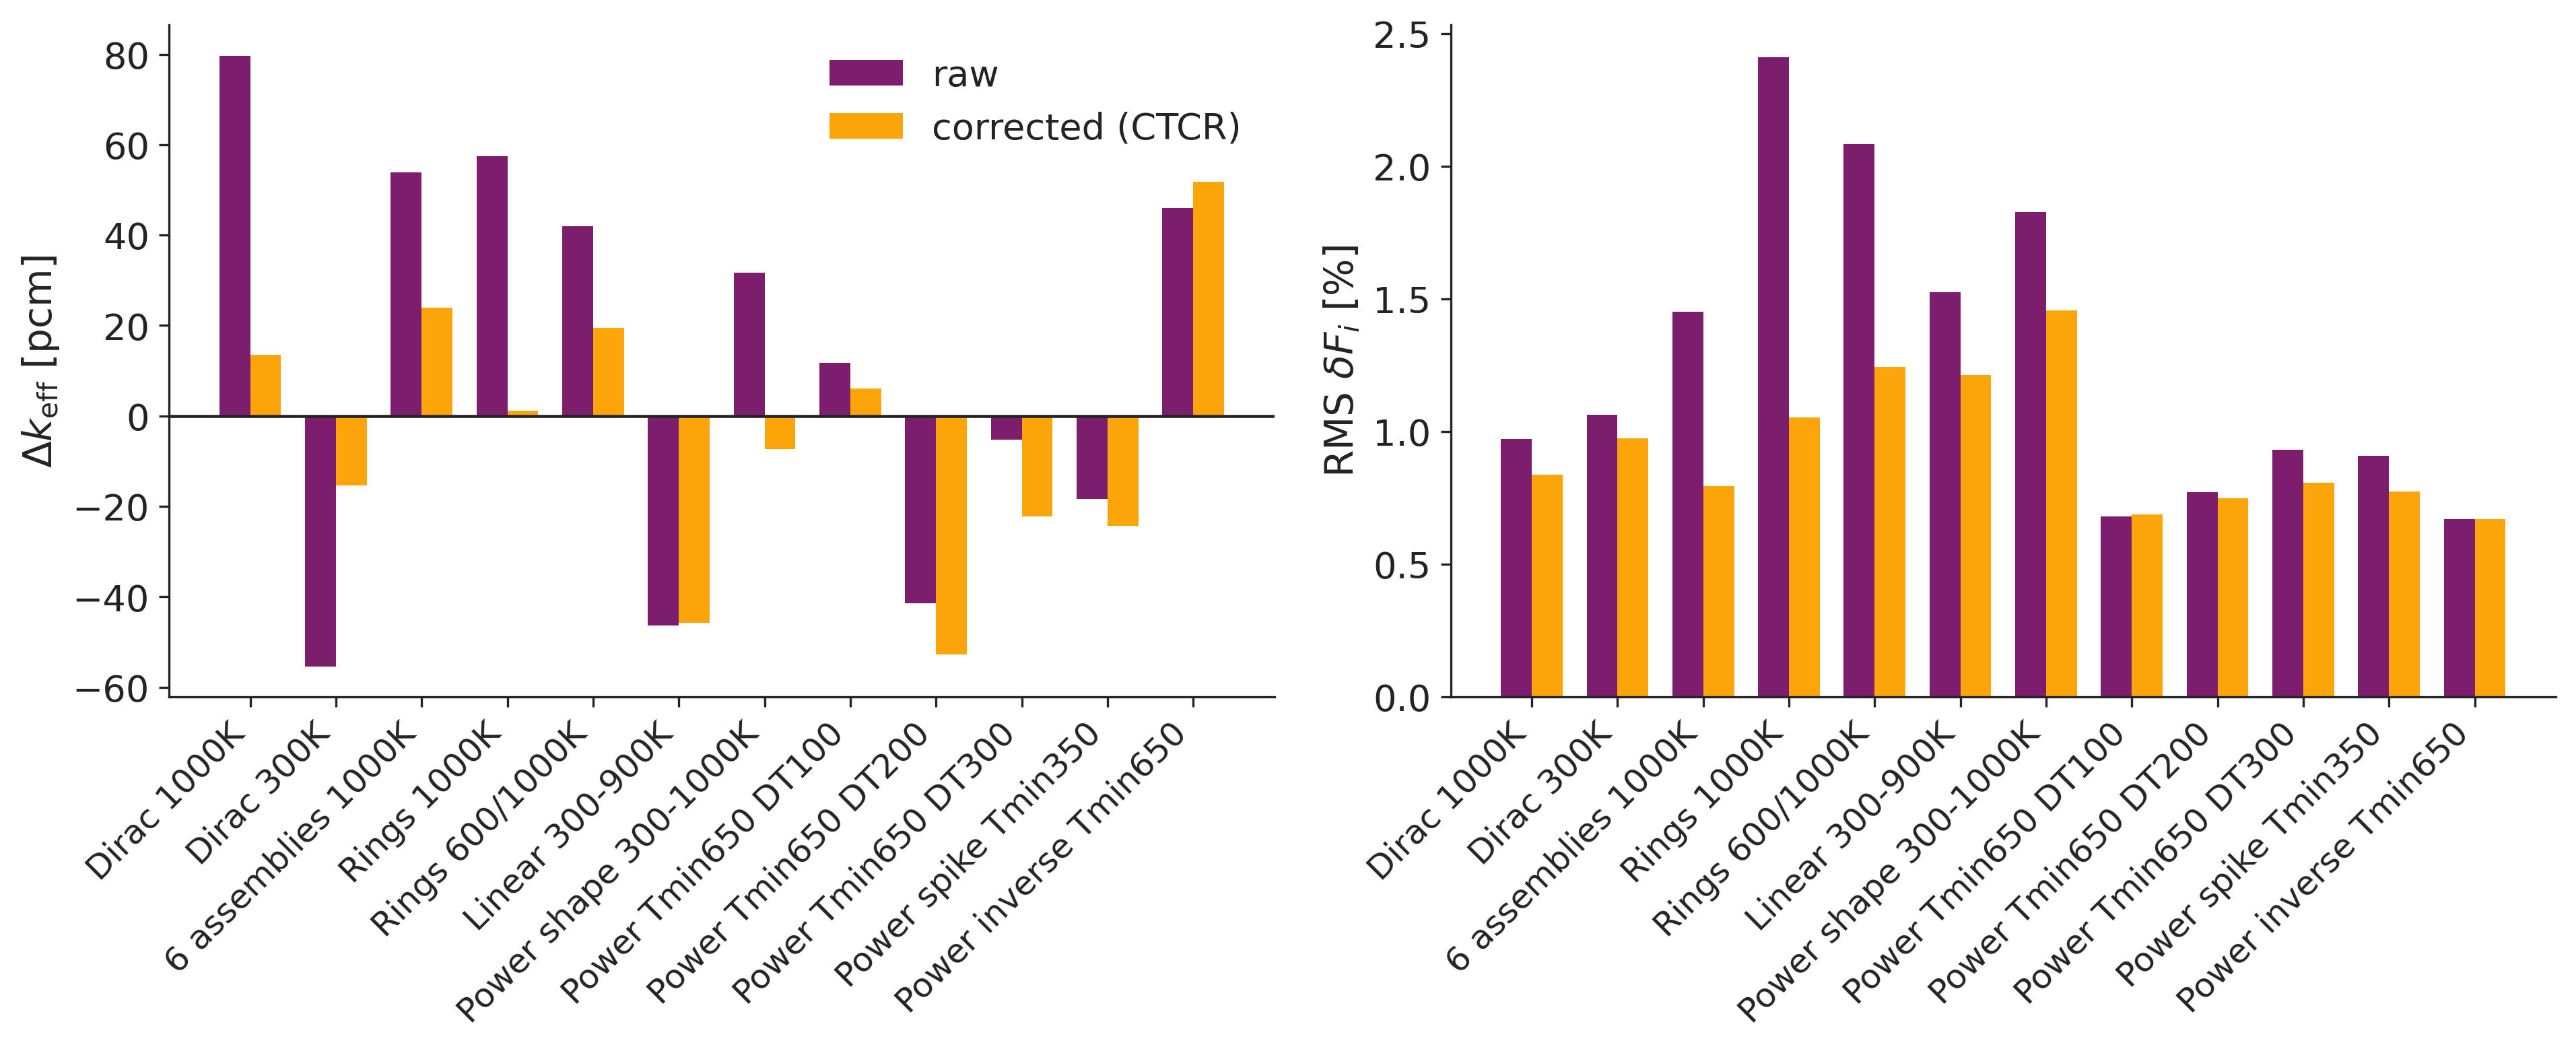
\includegraphics[width=140mm]{figures/fig3_raw_vs_corrected.png}
  \caption{$k_{\text{eff}}$ discrepancy (left) and fission-source RMS discrepancy (right), raw vs.\ CTCR-corrected interpolation, all twelve cases, with no uncertainty band.}
  \label{fig:fig3}
\end{figure}

\subsection{Combined Uncertainty}
\label{sec:res_final}

Combining $\sigma_{\text{ref}}$ (Sec.~\ref{sec:res_reference}) with $\sigma_{\text{database}}$ from the analytical model (Sec.~\ref{sec:validation}) in quadrature gives the total uncertainty $\sigma_{\text{tot}}$ of Eq.~(\ref{eqn:sigma_tot}). Under this combined budget, 58\% of the corrected cases fall within $|z|<2$ (median $|z|=1.30$), against 42\% of the raw cases (median $|z|=2.18$): a consistent and, for the corrected variant, now a majority of cases. $\sigma_{\text{database}}$ is 14--22~pcm against 9--12~pcm for $\sigma_{\text{ref}}$ in every case, so the database term still dominates the budget and both variants are judged against a relatively wide band.

Rather than collapsing this budget to a single $\pm2\sigma_{\text{tot}}$ number per case, Figure~\ref{fig:fig4} shows the full picture for $k_{\text{eff}}$: every one of the $N=500$ analytical-model realizations (gray) and, since 150 genuinely independent brute-force replicas of the whole database already exist (Sec.~\ref{sec:four_methods}), every one of those true replicas too (blue open circles), alongside the reference case's own $\pm2\sigma_{\text{ref}}$ (pink band) and the raw/corrected point estimates (black/red). Collapsing this to a single reported standard deviation, as in a conventional error-bar plot, would hide \emph{where} a case's point estimate actually falls within its own uncertainty: a case can sit near the edge of its distribution, or comfortably at its center, and only the full cloud shows which.

For the fission source (Figs.~\ref{fig:fig5}--\ref{fig:fig5b}) the same full-distribution logic is applied differently, for two reasons specific to this observable. First, at 127 zones per case the $N=500$ synthetic analytical realizations add visual clutter without adding information beyond what Sec.~\ref{sec:validation} already establishes about that model's accuracy, so only the $N=150$ genuine, independent brute-force replicas (Track A, no resampling assumption at all) are shown, split by flavor: raw in gray, corrected in shades of red. Second, every point --- ensemble and point estimate alike --- is tested directly against the reference case's own $\pm2\sigma_{\text{ref}}$, drawn here as its true, zone-by-zone curve (dashed black lines) rather than folded into a single reported number as in Fig.~\ref{fig:fig4}. A corrected point is recolored gold if and only if it falls inside that band \emph{and} the matching raw point --- same zone, same replica --- was outside it: exactly the population for which the CTCR turned a discrepancy raw could not explain by noise into one it can. Every other corrected point --- already consistent with noise in raw, or still not explained by noise even after correction --- keeps the base red. This isolates the population the correction is meant to act on, rather than diluting the plot with every in-band point regardless of whether raw needed fixing there at all.

\begin{figure}[t]
  \centering
  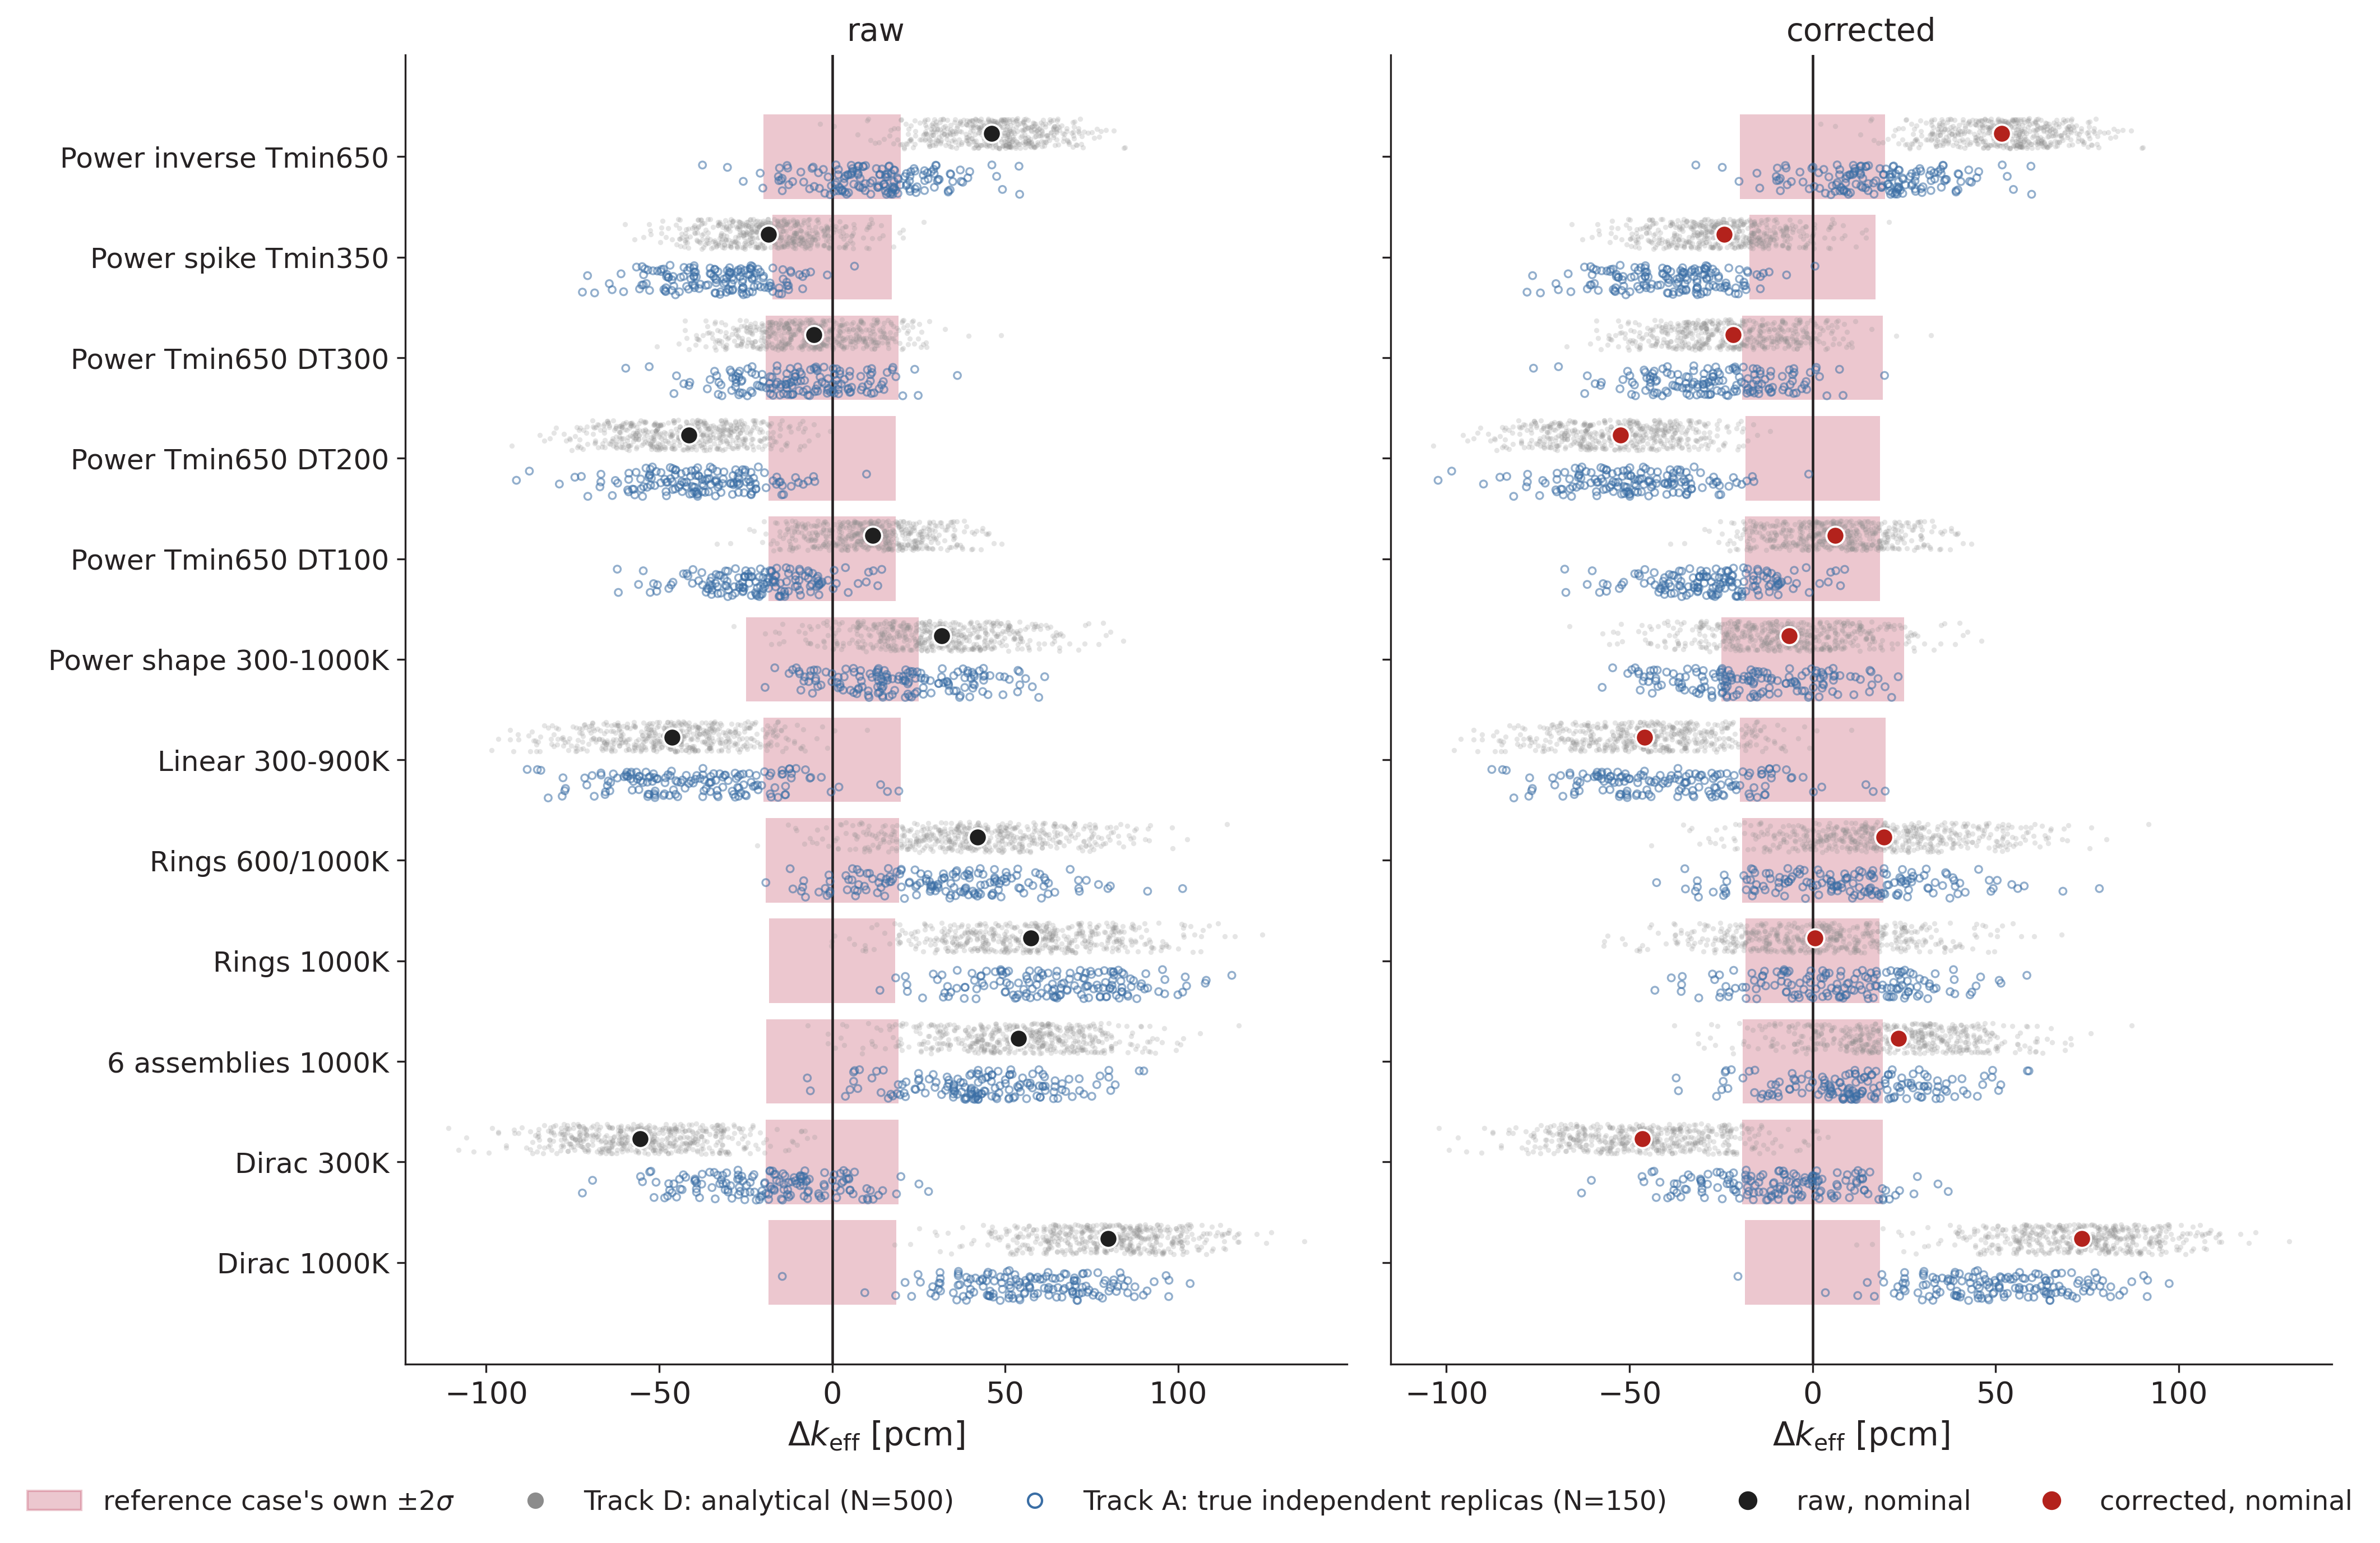
\includegraphics[width=150mm]{figures/fig4_keff_points_distribution_vs_truth_combined.png}
  \caption{$k_{\text{eff}}$ discrepancy, raw (left) and corrected (right): every analytical-model realization (gray, $N=500$) and every true independent brute-force replica (blue open circles, $N=150$), with the reference case's own $\pm2\sigma_{\text{ref}}$ (pink band) and the point estimate (filled circle), all twelve cases.}
  \label{fig:fig4}
\end{figure}

This systematic offset of the whole replica distribution away from zero is itself informative: it points to a mismatch between the database and some of the test cases that no amount of resampling the database can correct, because it is not database noise at all. The database is tallied with the radial reflector at the same uniform temperature as the rest of the core at each of its eight reference points, whereas several test cases instead fix the reflector at a constant 300~K regardless of the in-core field being tested. Where the in-core temperature departs from 300~K, this creates a sharp, systematic core-to-reflector gradient that is simply absent from the database's own construction, and every replica of that database --- brute-force or synthetic --- inherits the same mismatch, hence the same offset. This is a bias in the comparison's reference frame, not a statistical fluctuation, and no amount of resampling removes it.

Where the corrected replica cloud is centered close to zero --- Dirac 300~K, Linear 300--900~K, and most of the cases in Fig.~\ref{fig:fig5b} --- the residual deviation from the reference is statistically indistinguishable from Monte Carlo noise (and the reflector-mismatch bias just described, where present, is small relative to that noise), and no further correction is warranted. Where it is not --- the localized spikes in Dirac 1000~K, 6-assemblies 1000~K, and the Rings cases --- the deviation exceeds what either noise source can account for, and is therefore a genuine, uncorrected bias rather than statistical scatter. Because the database-noise model has itself been validated against brute force (Sec.~\ref{sec:validation}), it is not the plausible origin of these residuals; the most likely cause is the interpolation scheme's finite temperature grid, whose eight-point spacing cannot fully resolve the sharpest gradients. Figure~\ref{fig:hex_map} maps each zone index in Figs.~\ref{fig:fig5}--\ref{fig:fig5b} back to its physical hexagon.

A global summary metric can be misleading about how well the correction is actually doing its job locally. Sec.~\ref{sec:res_raw_vs_corrected} already reported the CTCR's benefit on the two aggregate figures of merit, $k_{\text{eff}}$ and the fission-source RMS: both improve, but a global metric averages over all 127 zones, and so cannot distinguish a case that improves a little everywhere from one that improves dramatically in exactly the zone that matters and not at all elsewhere. Table~\ref{tab:hexcount} makes the zone-by-zone picture concrete on a per-case basis: for each of the twelve cases, the number of zones (out of 127) whose fission-source point estimate is statistically consistent with noise ($|\delta F_i|<2\sigma_{\text{tot}}$), raw versus corrected, under each of the four $\sigma_{\text{database}}$ models of Sec.~\ref{sec:four_methods}. The pattern mirrors the point-estimate result of Table~\ref{tab:reference_results}, but is sharper here: for the Rings cases the corrected count roughly doubles (e.g., Rings 1000~K rises from 36--41 to 77--88 zones out of 127, consistently across all four models), while for the smoothest profiles the shift is small or even mildly unfavorable (Dirac 300~K, Power Tmin650 DT100/DT200). This distinction matters beyond bookkeeping: for a transient analysis, where the quantity of interest is often a single, localized hot spot --- the most critical point of the system --- rather than any core-averaged figure, it is representativeness at that one zone, not how good the global $k_{\text{eff}}$ or the RMS looks on average, that determines whether the interpolated model can be trusted where an error would matter most.

\begin{table}[h]
\centering
\caption{Number of Zones (out of 127) Statistically Consistent with Noise ($|\delta F_i|<2\sigma_{\text{tot}}$), Raw (r) vs.\ Corrected (c), by Case and $\sigma_{\text{database}}$ Model}
\label{tab:hexcount}
\footnotesize
\begin{tabular}{lcccccccc}
\hline
 & \multicolumn{2}{c}{(i) Uncorr.} & \multicolumn{2}{c}{(ii) Analyt.} & \multicolumn{2}{c}{(iii) Meas.} & \multicolumn{2}{c}{(iv) Brute force} \\
Case & r & c & r & c & r & c & r & c \\ \hline
Dirac 1000~K            & 116 & 118 & 110 & 109 & 112 & 112 & 113 & 115 \\
Dirac 300~K              & 110 & 106 & 103 & 100 & 105 & 100 & 107 & 105 \\
6 assemblies 1000~K      & 103 & 114 & 102 & 103 & 103 & 106 & 103 & 112 \\
Rings 1000~K             &  41 &  84 &  36 &  77 &  37 &  79 &  40 &  88 \\
Rings 600/1000~K         &  55 &  87 &  51 &  85 &  55 &  85 &  55 &  88 \\
Linear 300--900~K        &  66 &  90 &  62 &  82 &  65 &  88 &  66 &  89 \\
Power shape 300--1000~K  &  61 &  77 &  59 &  76 &  60 &  76 &  60 &  76 \\
Power Tmin650 DT100      & 118 & 116 & 115 & 114 & 116 & 114 & 117 & 115 \\
Power Tmin650 DT200      & 117 & 119 & 113 & 113 & 114 & 114 & 115 & 115 \\
Power Tmin650 DT300      &  97 & 104 &  96 & 101 &  93 & 102 &  97 & 103 \\
Power spike Tmin350      & 109 & 109 & 101 & 106 & 103 & 107 & 107 & 107 \\
Power inverse Tmin650    & 120 & 119 & 114 & 115 & 117 & 116 & 117 & 116 \\ \hline
\end{tabular}
\end{table}

\begin{figure}[t]
  \centering
  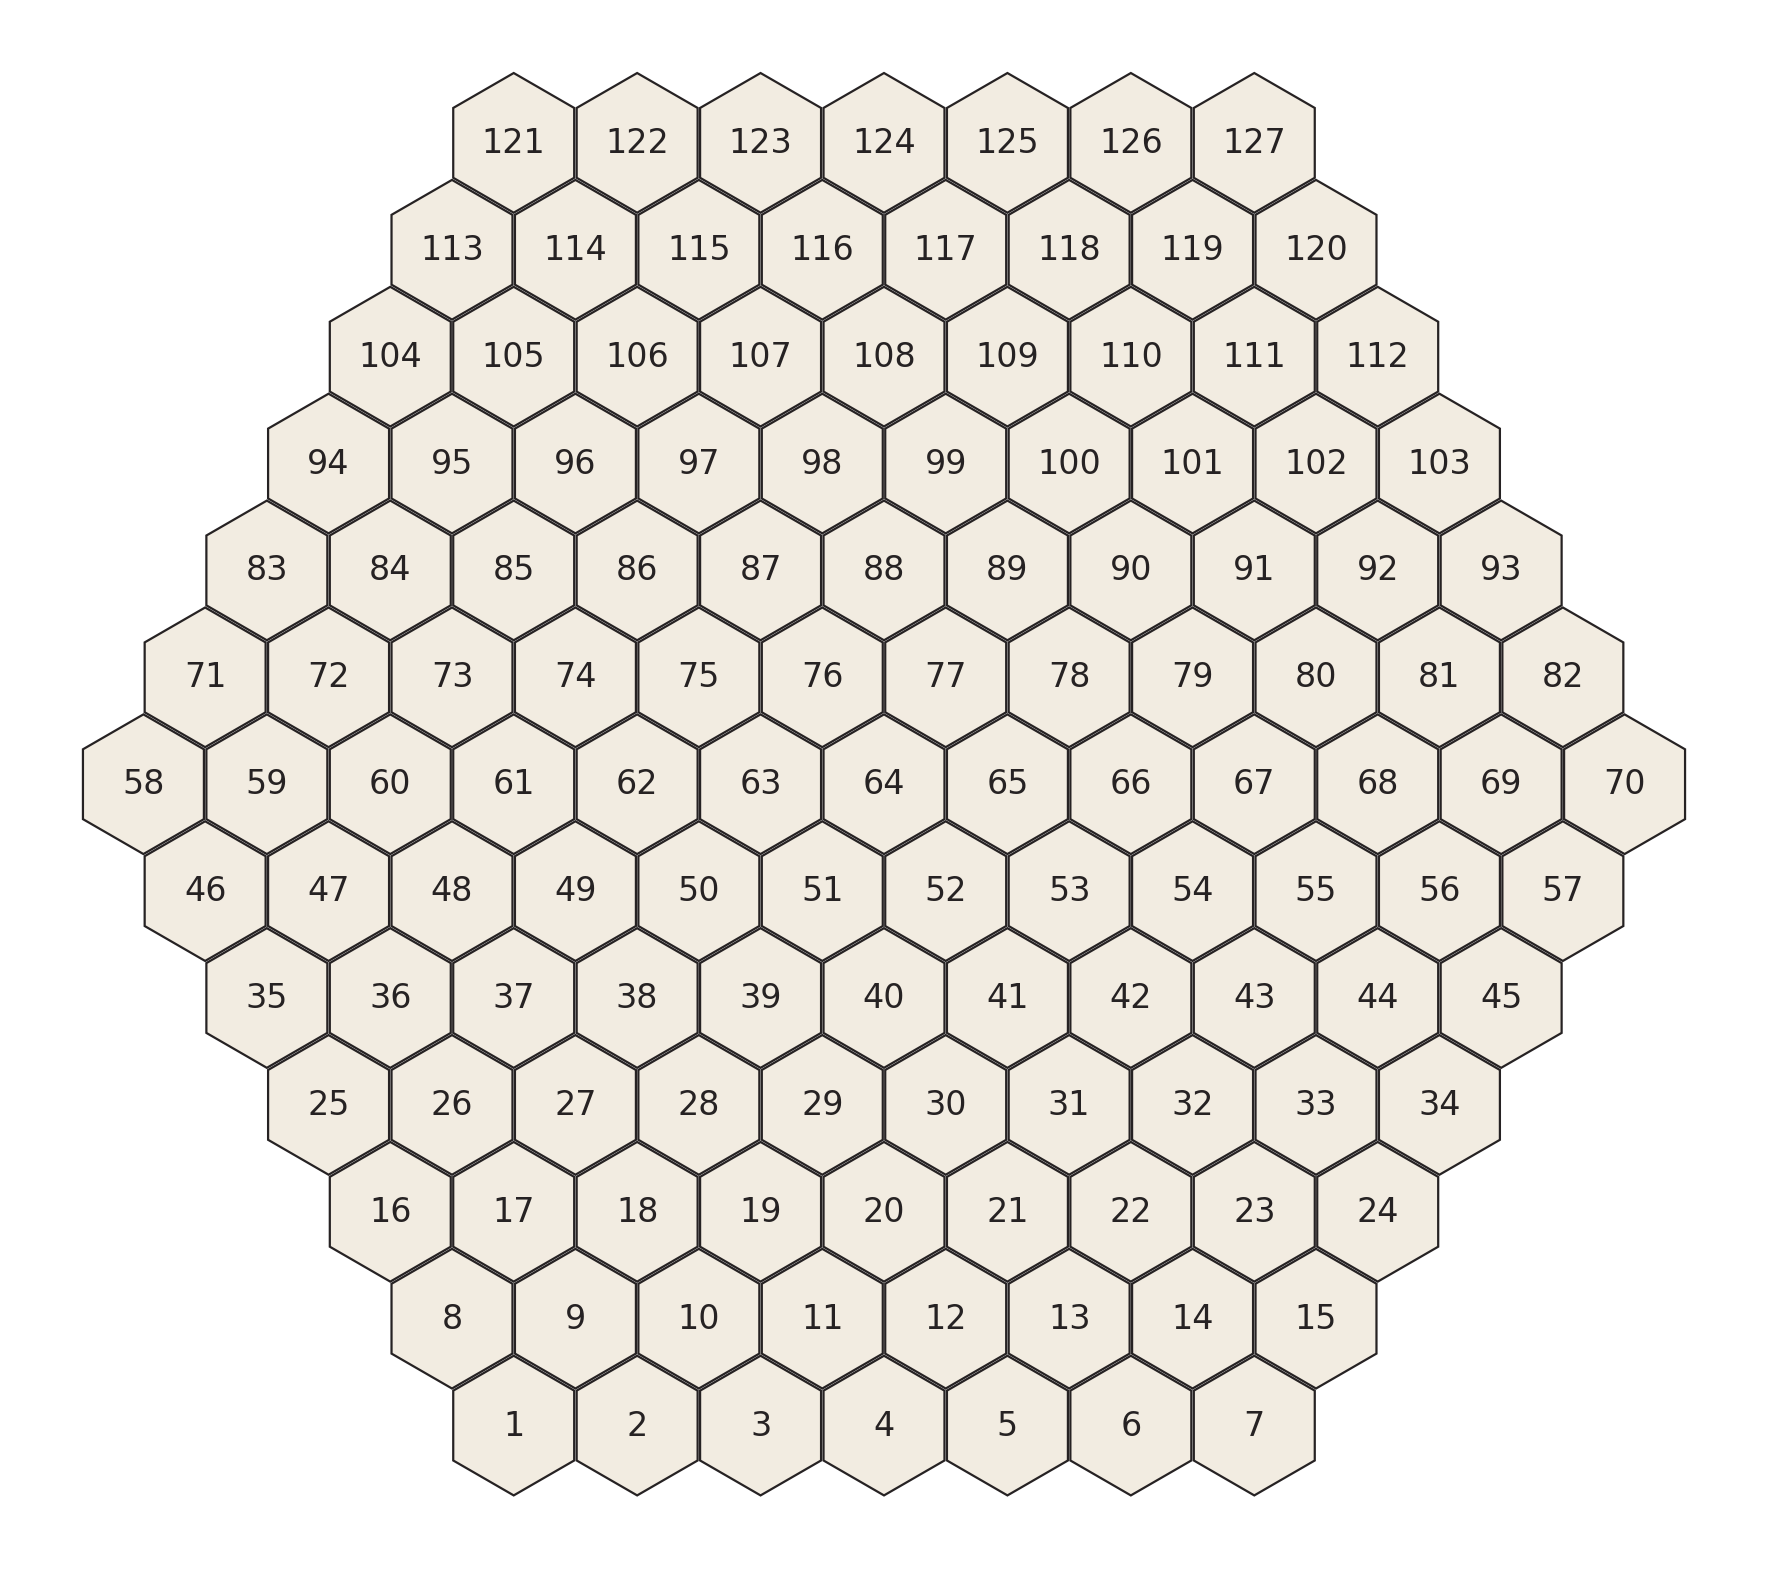
\includegraphics[width=110mm]{figures/hex_index_map.png}
  \caption{Hexagon-index map (1--127) referenced by the zone-index axis of Figs.~\ref{fig:fig5}--\ref{fig:fig5b}; hexagon 64 is the central assembly $C$ of the Dirac calibration cases (Sec.~\ref{sec:pipeline}).}
  \label{fig:hex_map}
\end{figure}

\begin{figure}[t]
  \centering
  \includegraphics[width=150mm]{figures/fig5a_fission_source_brute_force_rescue.png}
  \caption{Fission-source relative deviation from the reference, zone by zone, true brute-force replicas only (Track A, $N=150$, no resampling assumption): raw ensemble (gray) and corrected ensemble (red, or gold where ``rescued''), together with the raw (black, filled) and corrected (dark red, or gold where rescued) point estimates, and the reference case's own $\pm2\sigma_{\text{ref}}$ drawn as its true zone-by-zone curve (dashed black lines) rather than a single flattened value. A corrected point --- ensemble replica or point estimate --- is colored gold precisely when it falls inside this band \emph{and} the matching raw point (same zone, same replica) was outside it, i.e., where the correction turned a discrepancy raw could not explain by noise into one it can; every other corrected point keeps the base red. Test cases 1--6.}
  \label{fig:fig5}
\end{figure}

\begin{figure}[t]
  \centering
  \includegraphics[width=150mm]{figures/fig5b_fission_source_brute_force_rescue.png}
  \caption{As Fig.~\ref{fig:fig5}, for test cases 7--12.}
  \label{fig:fig5b}
\end{figure}


% \section{Results}
% \label{sec:results}

% All results use the 12 validation cases of Ref.~\cite{VitaPHYSOR2026}: two spatially sharp ``Dirac'' perturbations, a 6-assembly and two ring-shaped hot-spot patterns, a linear gradient, and six power-shaped profiles of varying sharpness and offset.

% \subsection{Reference-Case Uncertainty}
% \label{sec:res_reference}

% Figure~\ref{fig:fig1} shows $\sigma_{\text{ref}}$, source (a) of Sec.~\ref{sec:uncertainty}, on its own: a mean of 9.7~pcm on $k_{\text{eff}}$ and 0.309\% (RMS) on the fission source across the 12 cases, both essentially uniform except for the Power shape 300--1000~K case (12.5~pcm, 0.42\%), whose broader and shallower temperature profile yields a less peaked, statistically noisier fission-source detector tally. This is only half the noise budget: it says nothing about the uncertainty the interpolation itself introduces.

% \begin{figure}[t]
%   \centering
%   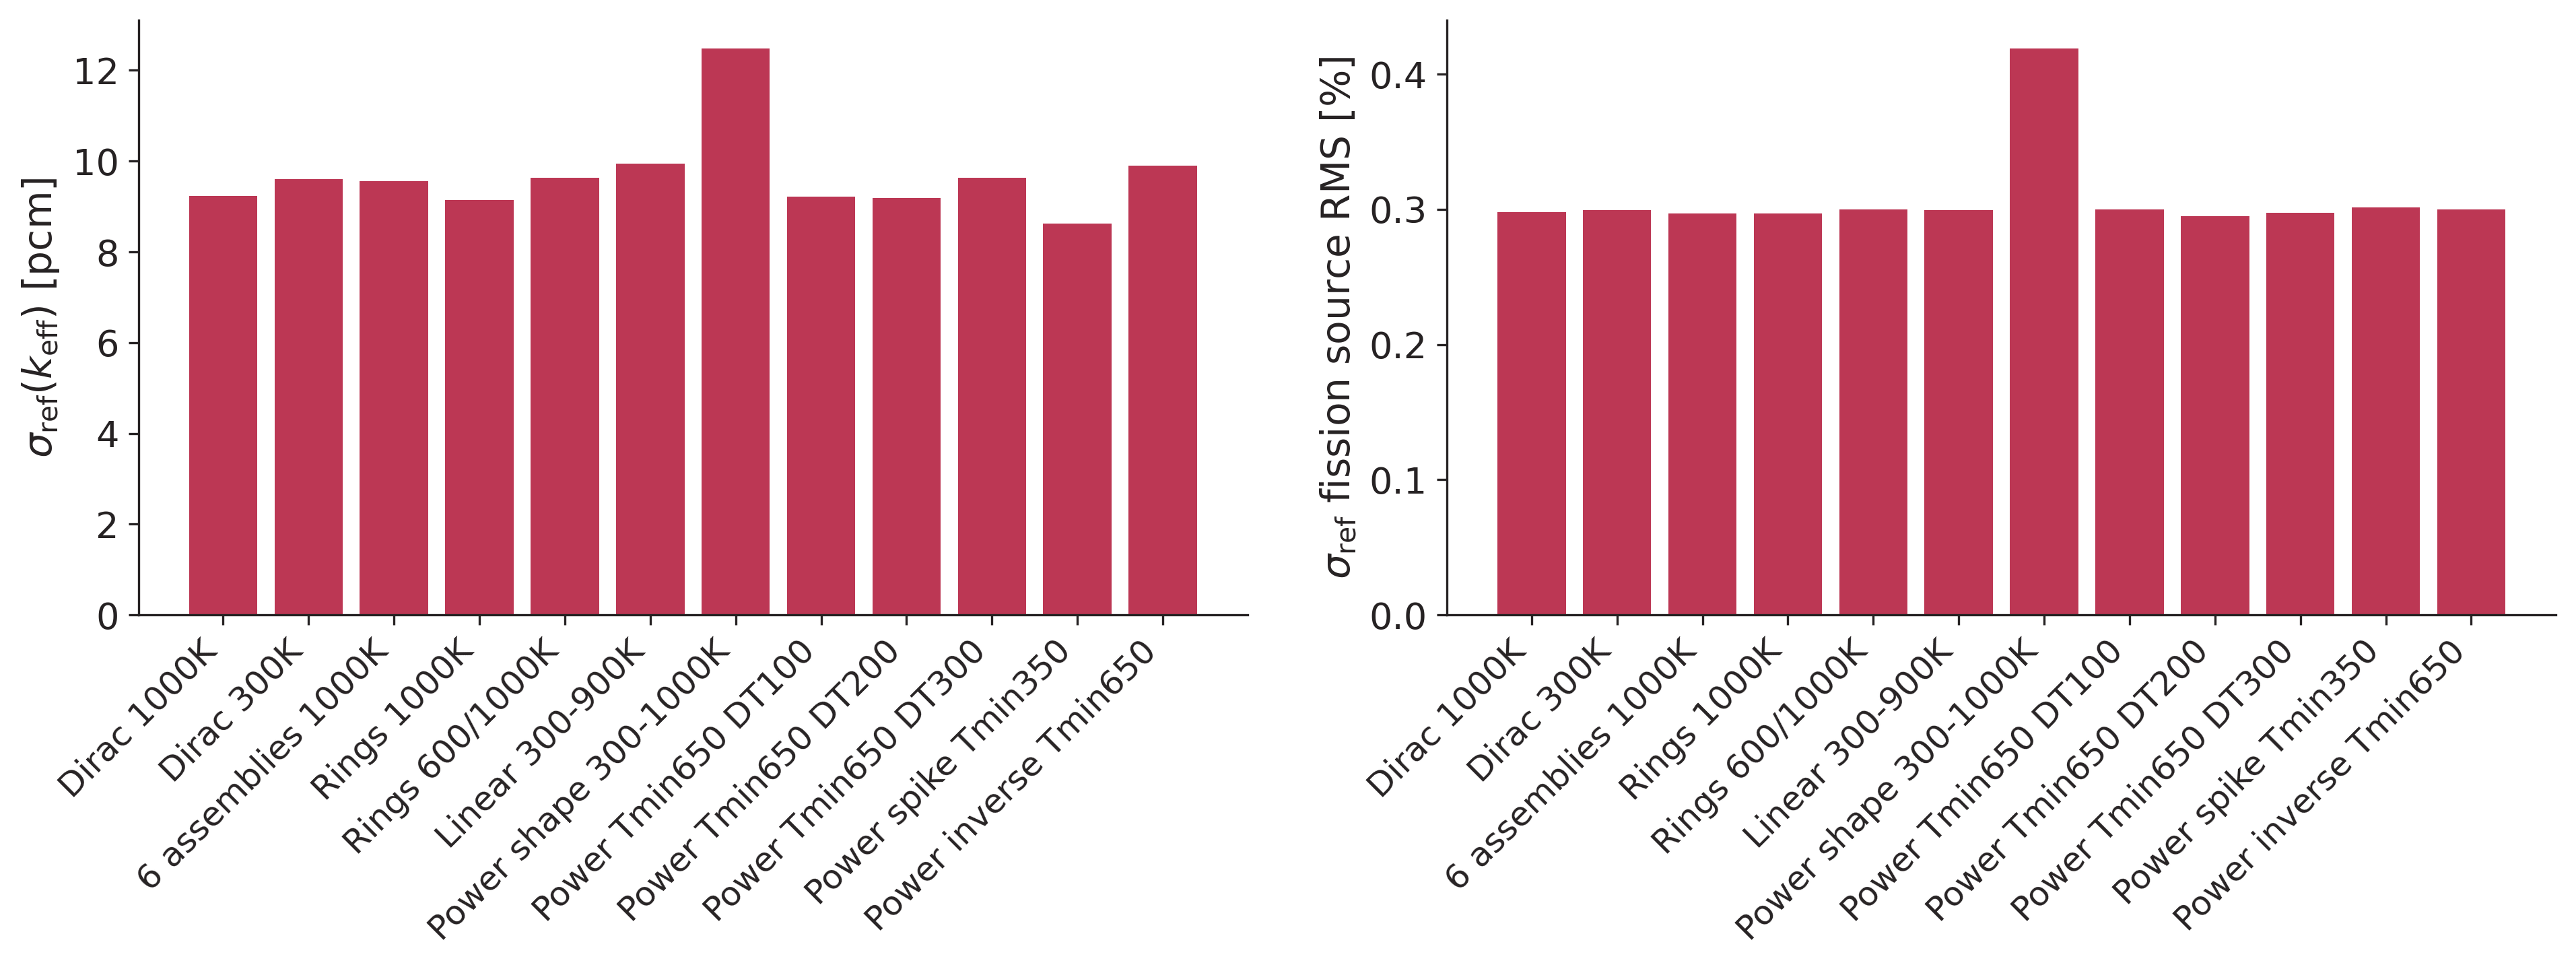
\includegraphics[width=140mm]{figures/fig1_reference_case_uncertainty.png}
%   \caption{Reference-case own MC uncertainty, $\sigma_{\text{ref}}$: $k_{\text{eff}}$ (left, from \texttt{\_res.m}) and fission-source RMS (right, from \texttt{\_det0.m}), all 12 cases.}
%   \label{fig:fig1}
% \end{figure}

% \subsection{Validating the Four Methods Against Brute Force}
% \label{sec:validation}

% Figure~\ref{fig:fig2} compares the three cheap approaches of Sec.~\ref{sec:four_methods} against the brute-force result, for the corrected variant of all 12 cases, on both $k_{\text{eff}}$ and the fission-source RMS. On $k_{\text{eff}}$, the analytical model reproduces the brute-force uncertainty with a mean absolute deviation of 4.6\% across the 12 cases, ahead of the single-seed correlated model (8.7\%) and the uncorrelated model (18.0\%), while requiring no MC replicas beyond the nominal database. On the fission-source RMS, the ranking is different: the uncorrelated (3.3\%) and single-seed correlated (3.6\%) models track brute force more closely than the analytical one (7.3\%). We nonetheless use the analytical model uniformly for both observables in Sec.~\ref{sec:res_final}, since it requires no additional simulation and is, on both observables, within the same order of magnitude as the more expensive alternatives --- adequate for the practical question this work asks, even though it is not uniformly the best of the three.

% \begin{figure}[t]
%   \centering
%   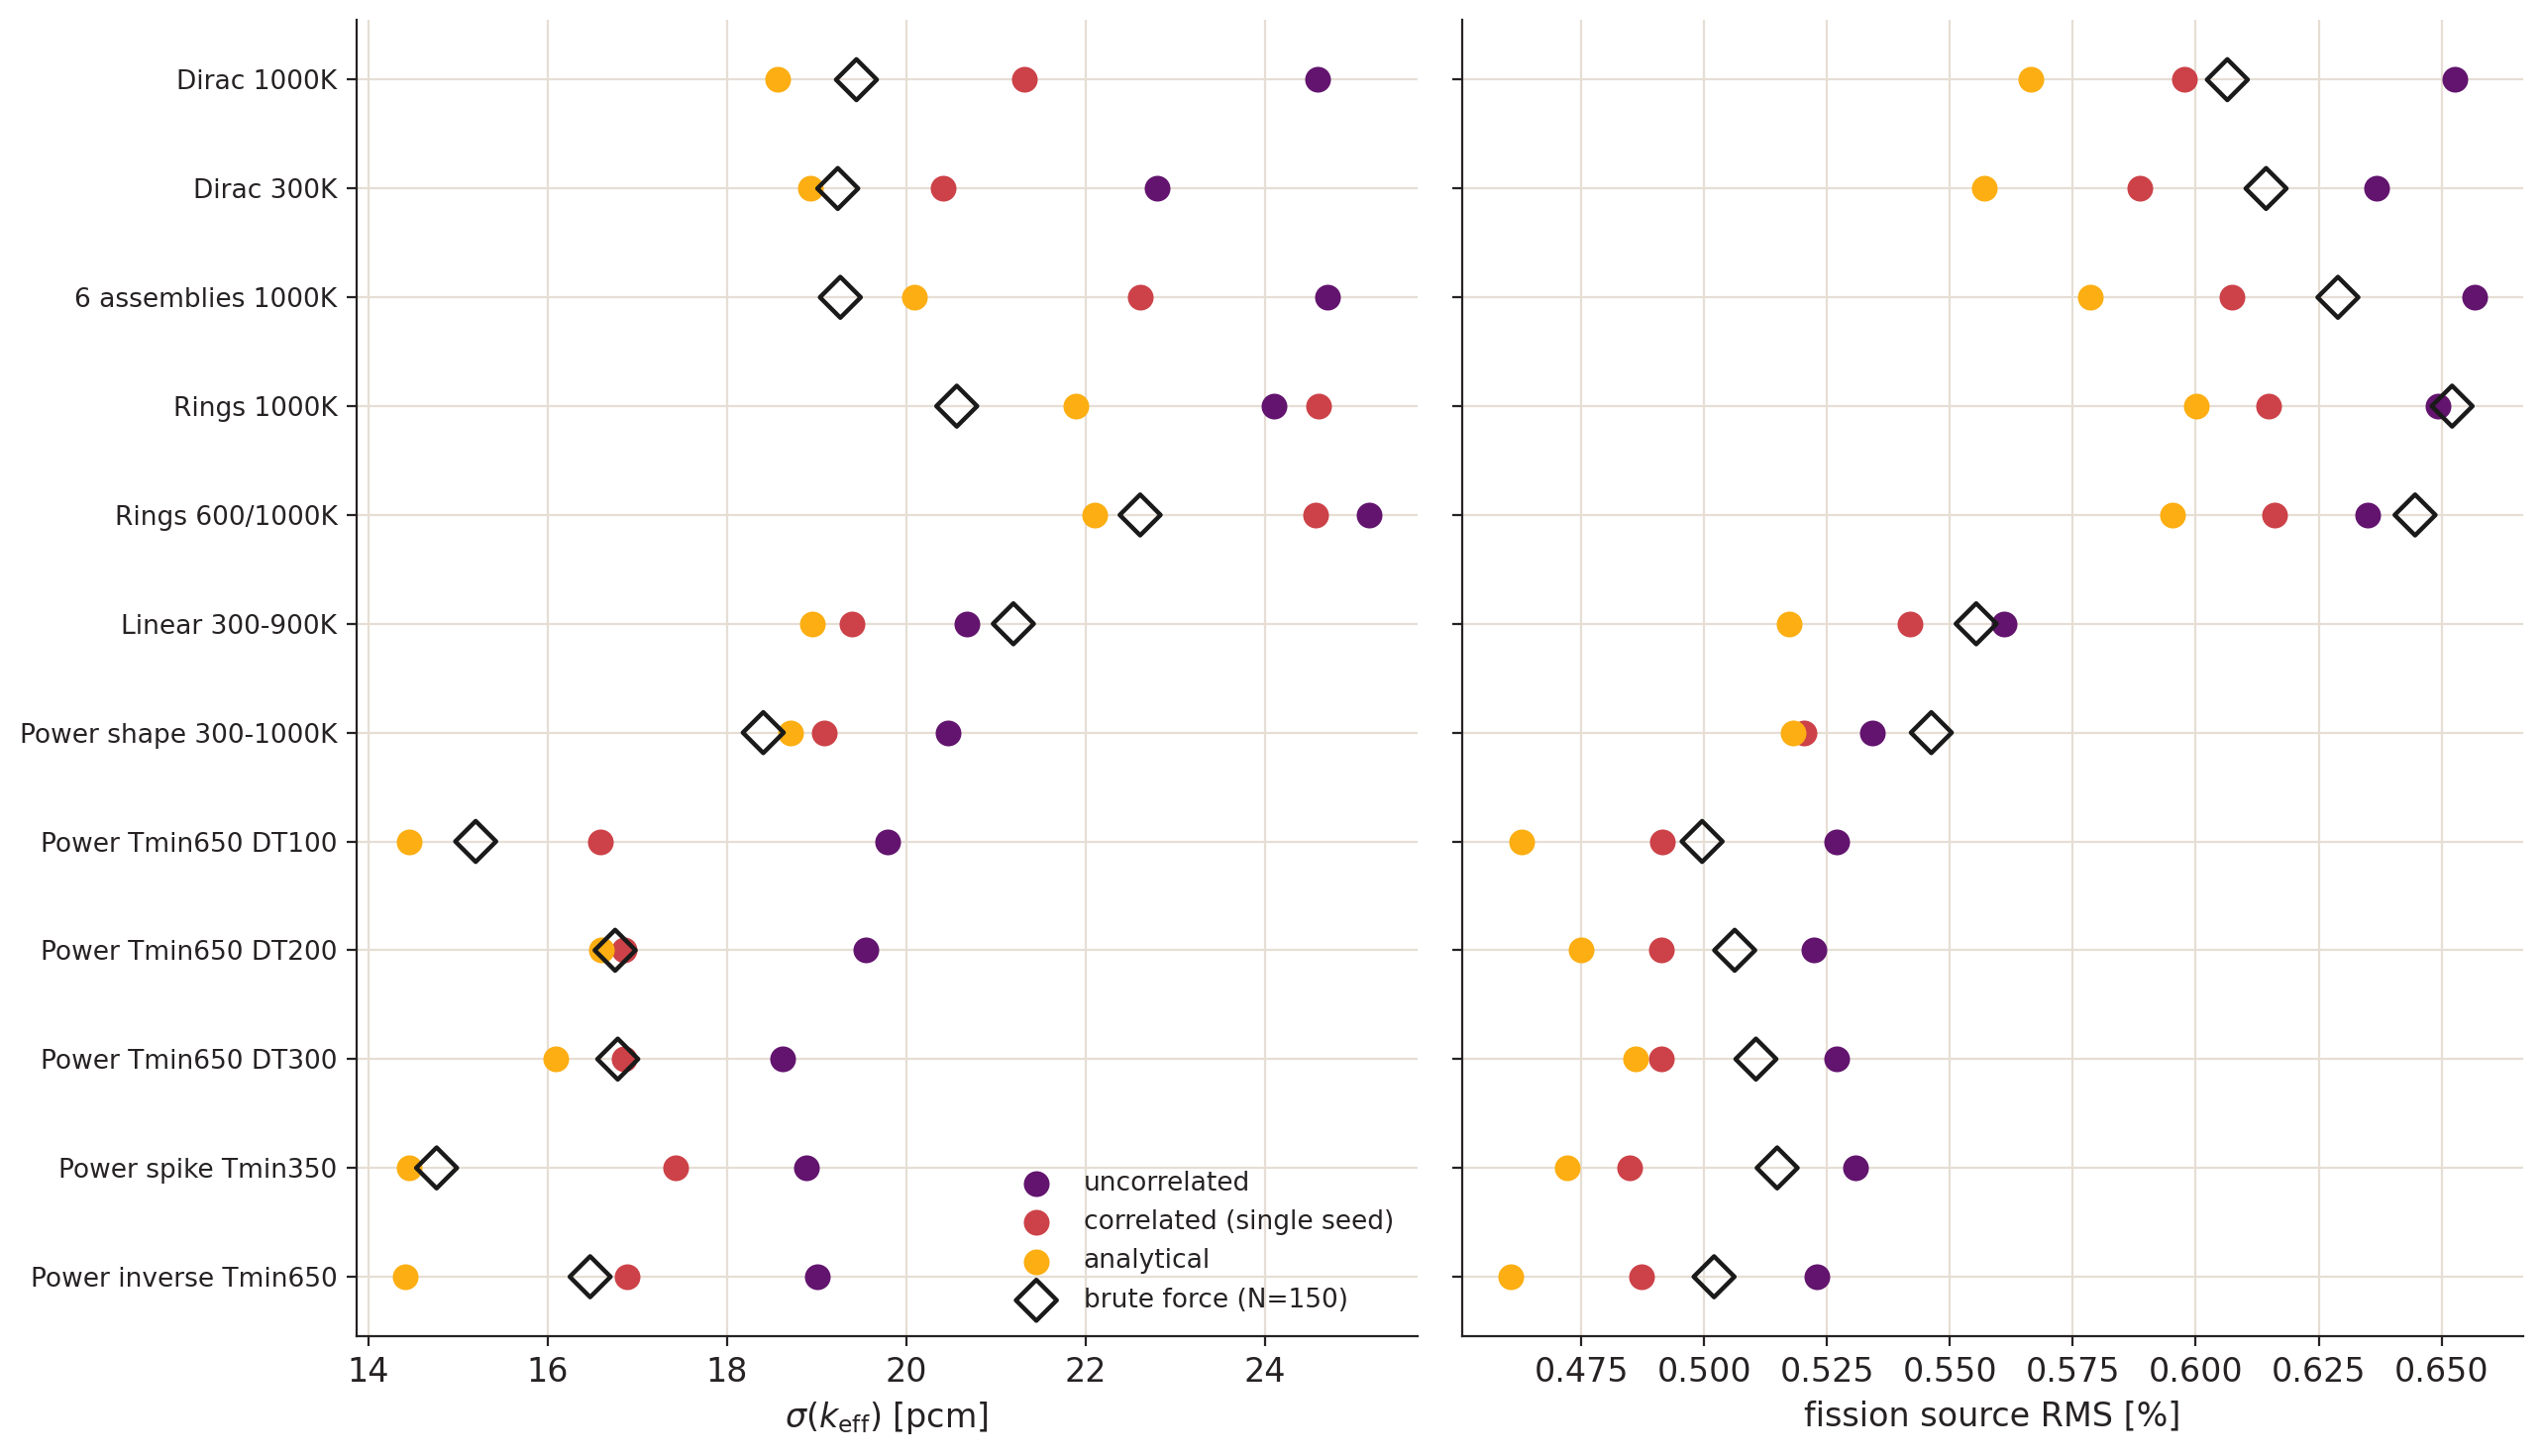
\includegraphics[width=140mm]{figures/fig2_validation_against_brute_force.png}
%   \caption{Predicted database-side uncertainty under methods (i)--(iii) of Sec.~\ref{sec:four_methods} vs.\ the brute-force result (iv, $N=150$): $k_{\text{eff}}$ (left) and fission-source RMS (right), corrected variant, all 12 cases.}
%   \label{fig:fig2}
% \end{figure}

% \subsection{Does the Correction Ratio Help?}
% \label{sec:res_raw_vs_corrected}

% Figure~\ref{fig:fig3} compares raw and corrected interpolation against the direct reference, with no uncertainty consideration yet. Averaged over the 12 cases, the CTCR reduces the mean absolute $k_{\text{eff}}$ discrepancy from 40.8 to 36.9~pcm (10\%) and the mean fission-source RMS discrepancy from 1.27\% to 1.02\% (20\%). The benefit is markedly uneven: it is large for the sharpest, most spatially localized cases (e.g., Power shape 300--1000~K improves from $+31.7$ to $-7.0$~pcm; Rings 1000~K from $57.4$ to $28.8$~pcm), consistent with the CTCR's own calibration against a sharp central perturbation, but is negligible or mildly unfavorable for smoother, less localized profiles (e.g., Power Tmin650 DT200 worsens from $-41.5$ to $-52.7$~pcm), matching the geometric explanation given in Ref.~\cite{VitaPHYSOR2026}.

% \begin{figure}[t]
%   \centering
%   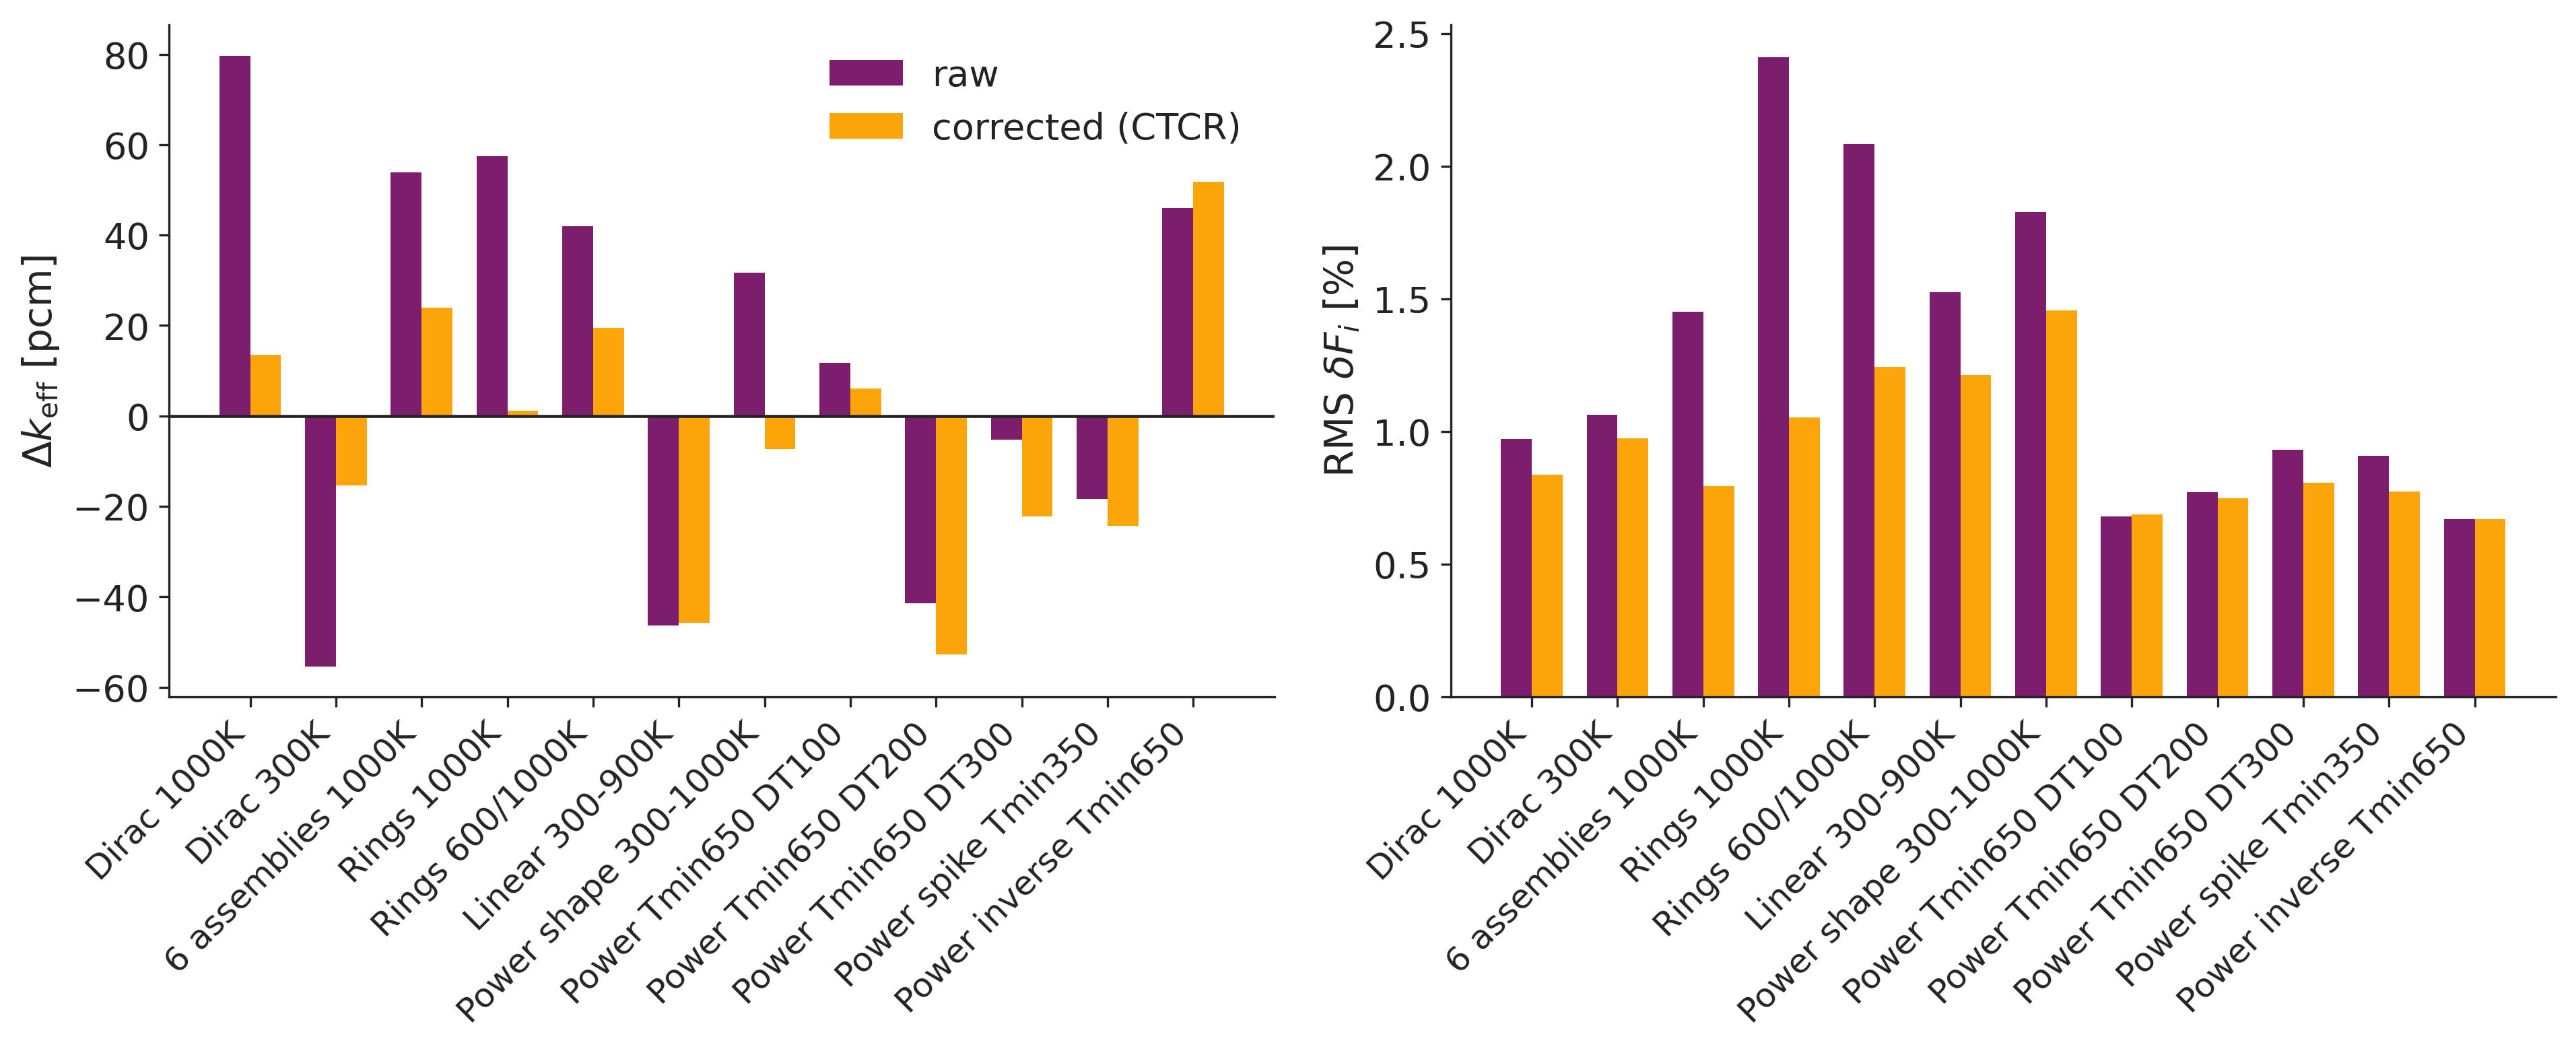
\includegraphics[width=140mm]{figures/fig3_raw_vs_corrected.png}
%   \caption{$k_{\text{eff}}$ discrepancy (left) and fission-source RMS discrepancy (right), raw vs.\ CTCR-corrected interpolation, all 12 cases, no uncertainty band.}
%   \label{fig:fig3}
% \end{figure}

% \subsection{Final Results: Combined Uncertainty Budget}
% \label{sec:res_final}

% Combining $\sigma_{\text{ref}}$ (Sec.~\ref{sec:res_reference}) with $\sigma_{\text{database}}$ from the analytical model (Sec.~\ref{sec:validation}) in quadrature gives $\sigma_{\text{tot}}$, shown as $\pm2\sigma_{\text{tot}}$ error bars in Fig.~\ref{fig:fig4} and as shaded $\pm2\sigma_{\text{tot}}$ bands in Fig.~\ref{fig:fig5}. Under this combined budget, $50\%$ of the corrected cases fall within $|z|<2$ (median $|z|=1.78$), against $42\%$ for the raw cases (median $|z|=2.17$): a modest but consistent improvement, smaller in this metric than the point-estimate reduction of Sec.~\ref{sec:res_raw_vs_corrected} because $\sigma_{\text{database}}$ (14--25~pcm) dominates $\sigma_{\text{ref}}$ (9--13~pcm) in every case, compressing the significance gap between the two variants.

% \begin{figure}[t]
%   \centering
%   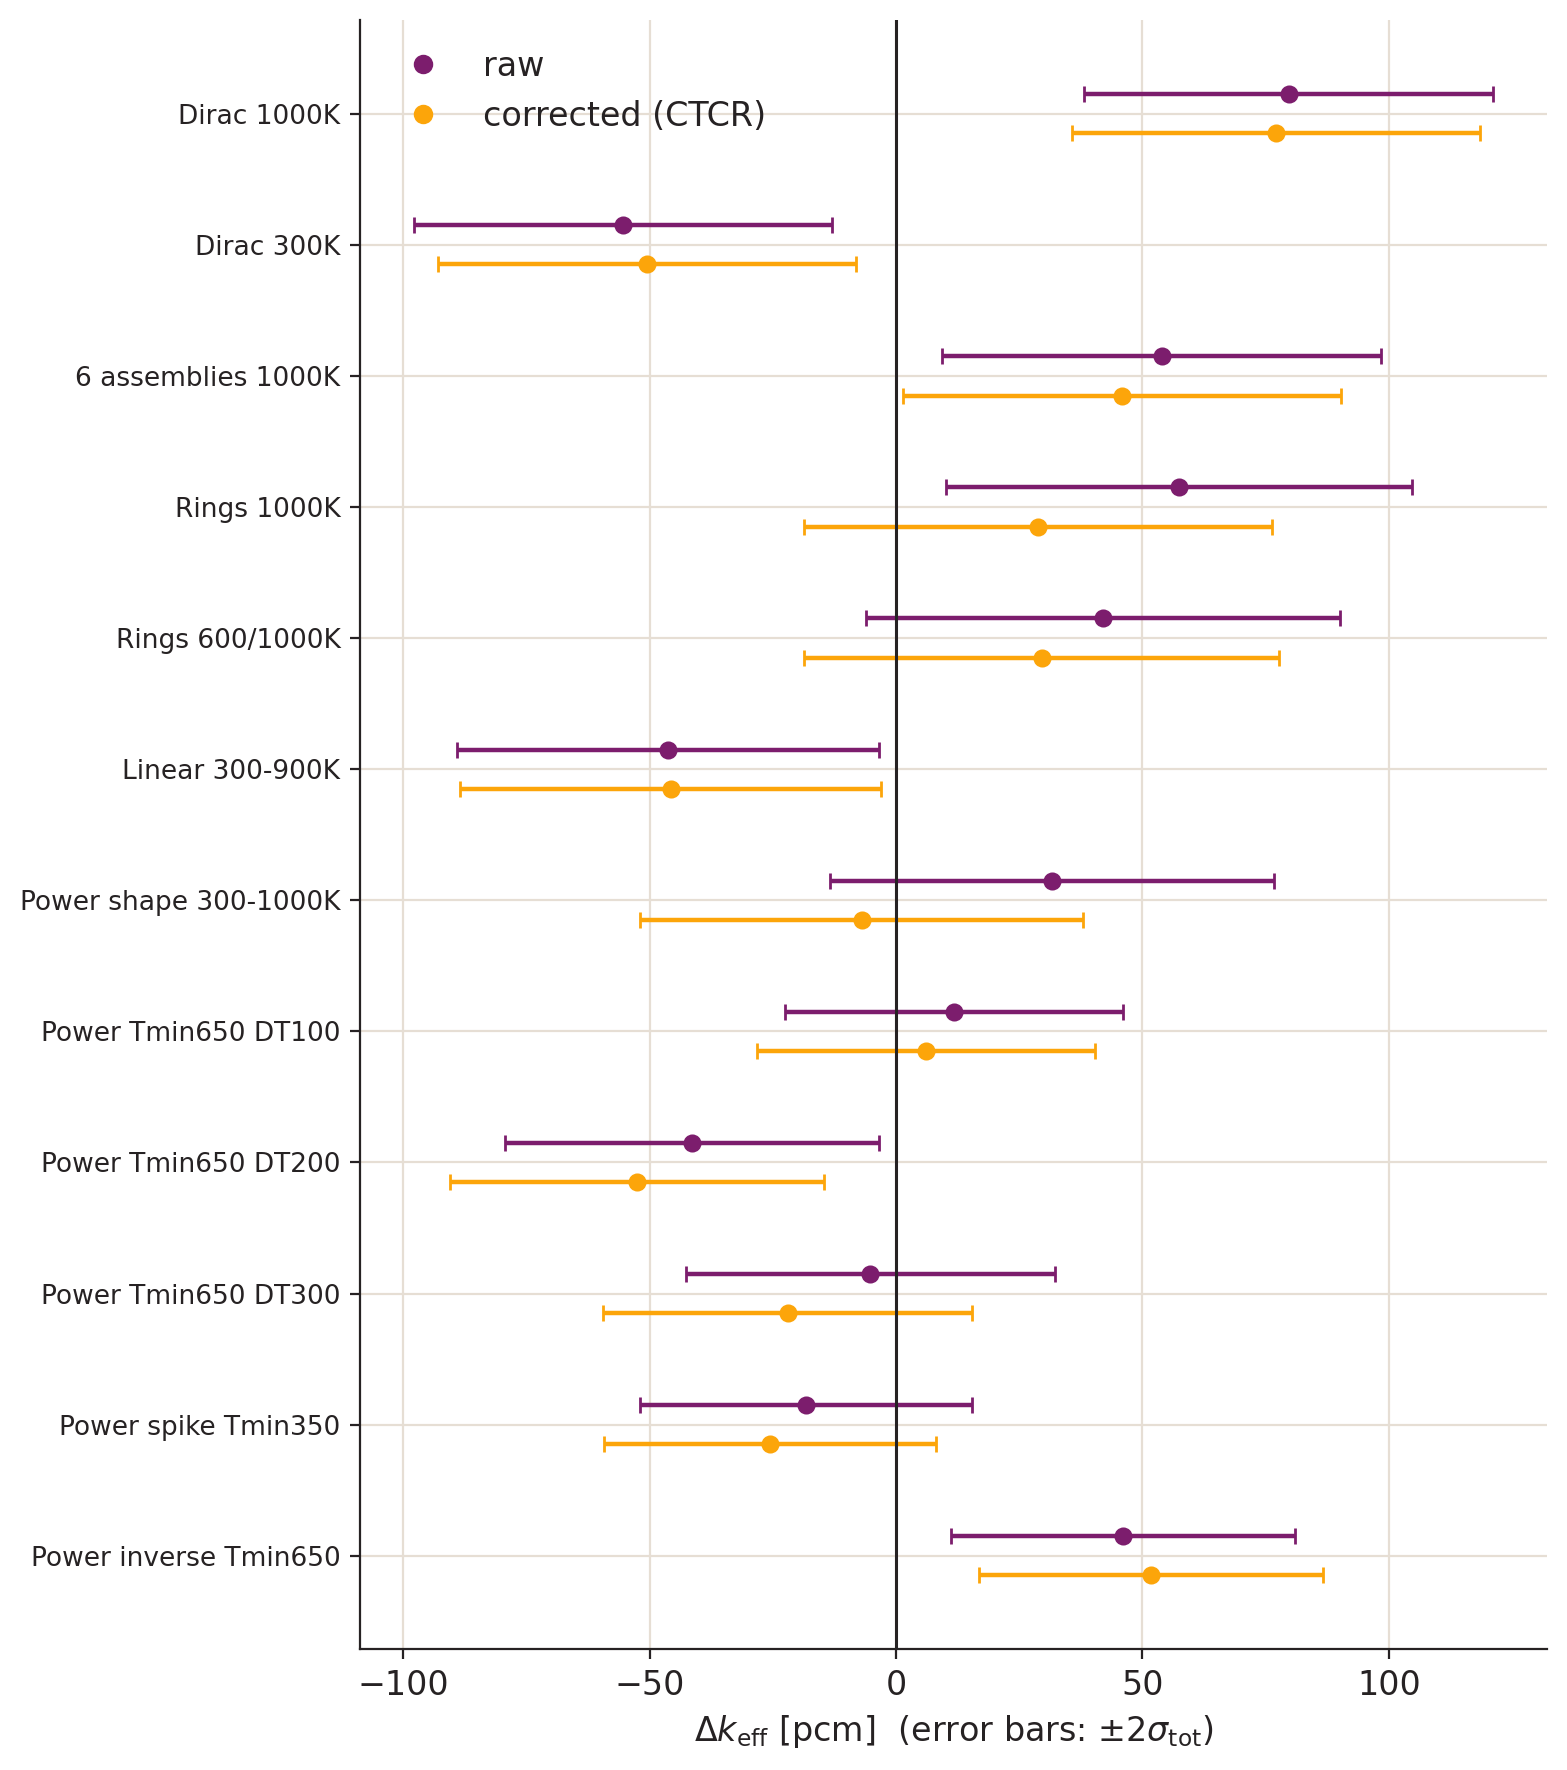
\includegraphics[width=110mm]{figures/fig4_keff_results.png}
%   \caption{$k_{\text{eff}}$ discrepancy with combined uncertainty $\pm2\sigma_{\text{tot}}$ (reference $\oplus$ analytical database model), matching the $|z|<2$ significance threshold, raw vs.\ corrected, all 12 cases.}
%   \label{fig:fig4}
% \end{figure}

% Figure~\ref{fig:fig5} shows the same combined budget spatially, zone by zone. Where the corrected line remains within its band (e.g., Dirac 300~K, Linear 300--900~K, most of Fig.~\ref{fig:fig5}b), the residual discrepancy is statistically indistinguishable from FM noise. Where it does not (e.g., the localized spikes in Dirac 1000~K, 6~assemblies 1000~K, and the Rings cases), the discrepancy exceeds what either noise source can explain, and is attributable to the interpolation scheme itself --- most plausibly the finite spacing of the 8-temperature grid --- rather than to the database-noise model, which is checked against brute force in Sec.~\ref{sec:validation} and therefore not, on its own, the source of this residual.

% \begin{figure}[t]
%   \centering
%   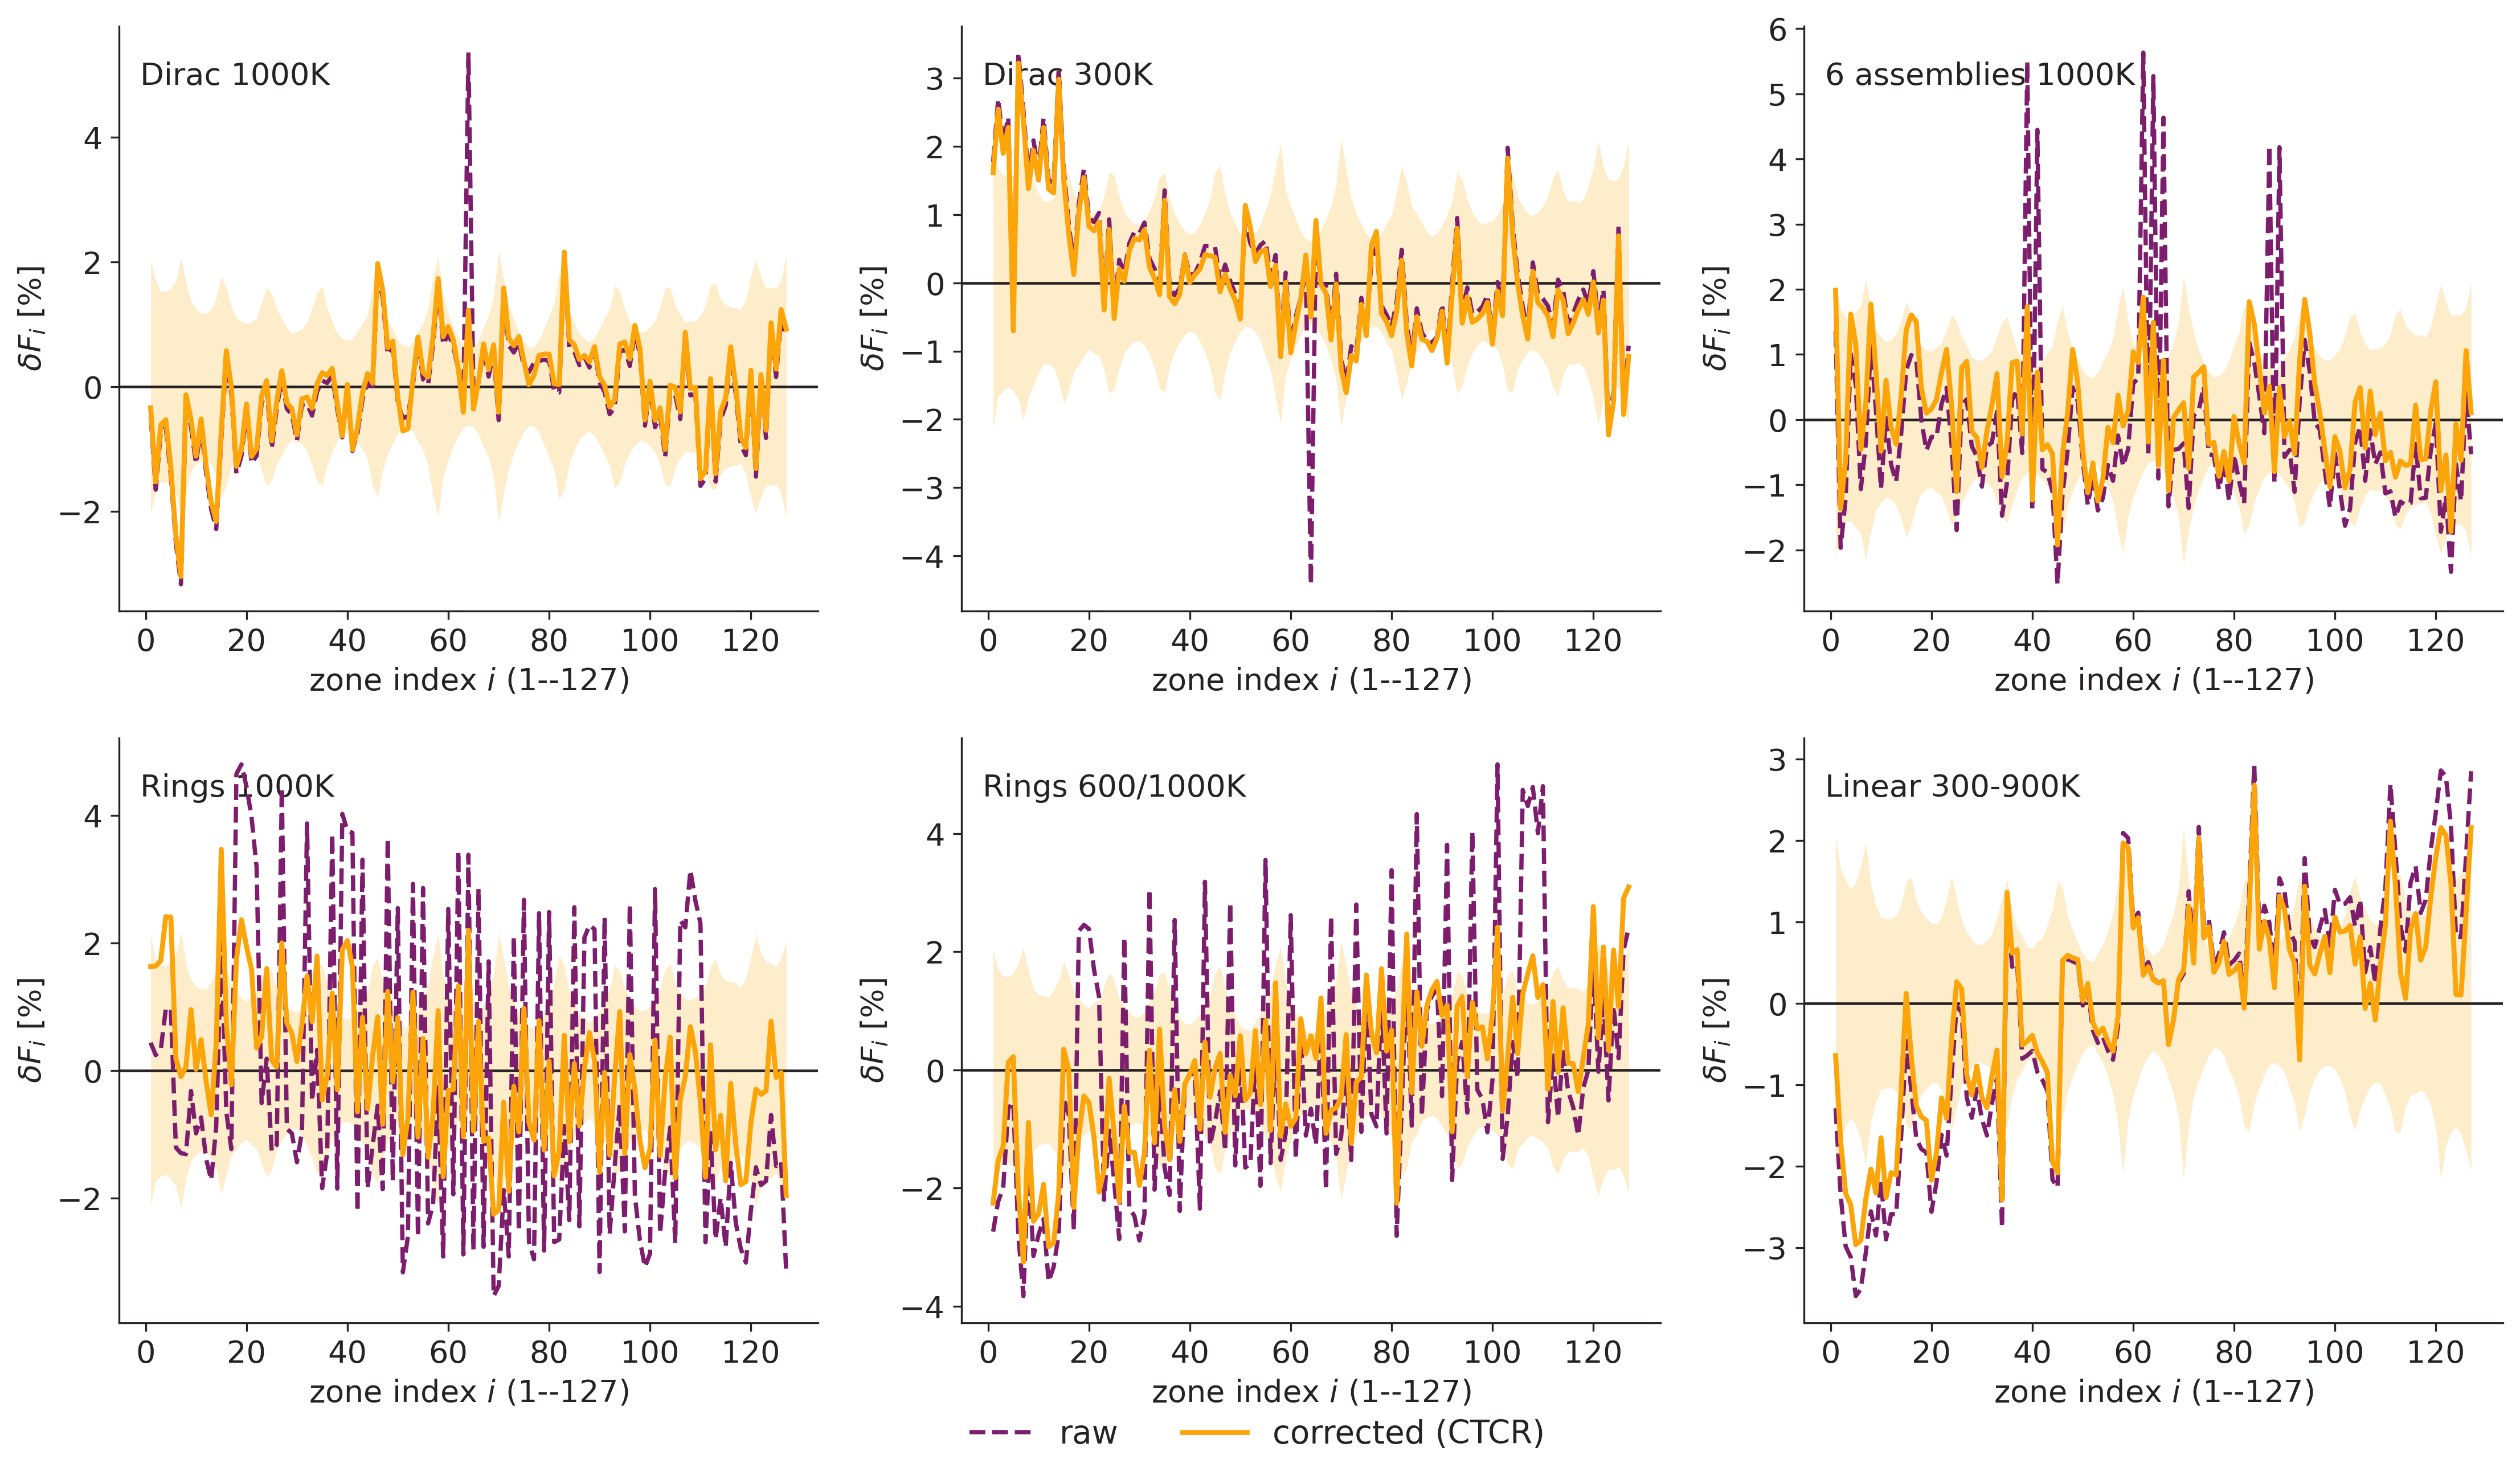
\includegraphics[width=140mm]{figures/fig5a_fission_source.png}
%   \caption{Fission-source relative deviation from reference, raw (dashed) vs.\ corrected (solid), with $\pm2\sigma_{\text{tot}}$ band (analytical model, corrected variant); Test Cases 1--6.}
%   \label{fig:fig5}
% \end{figure}

% \begin{figure}[t]
%   \centering
%   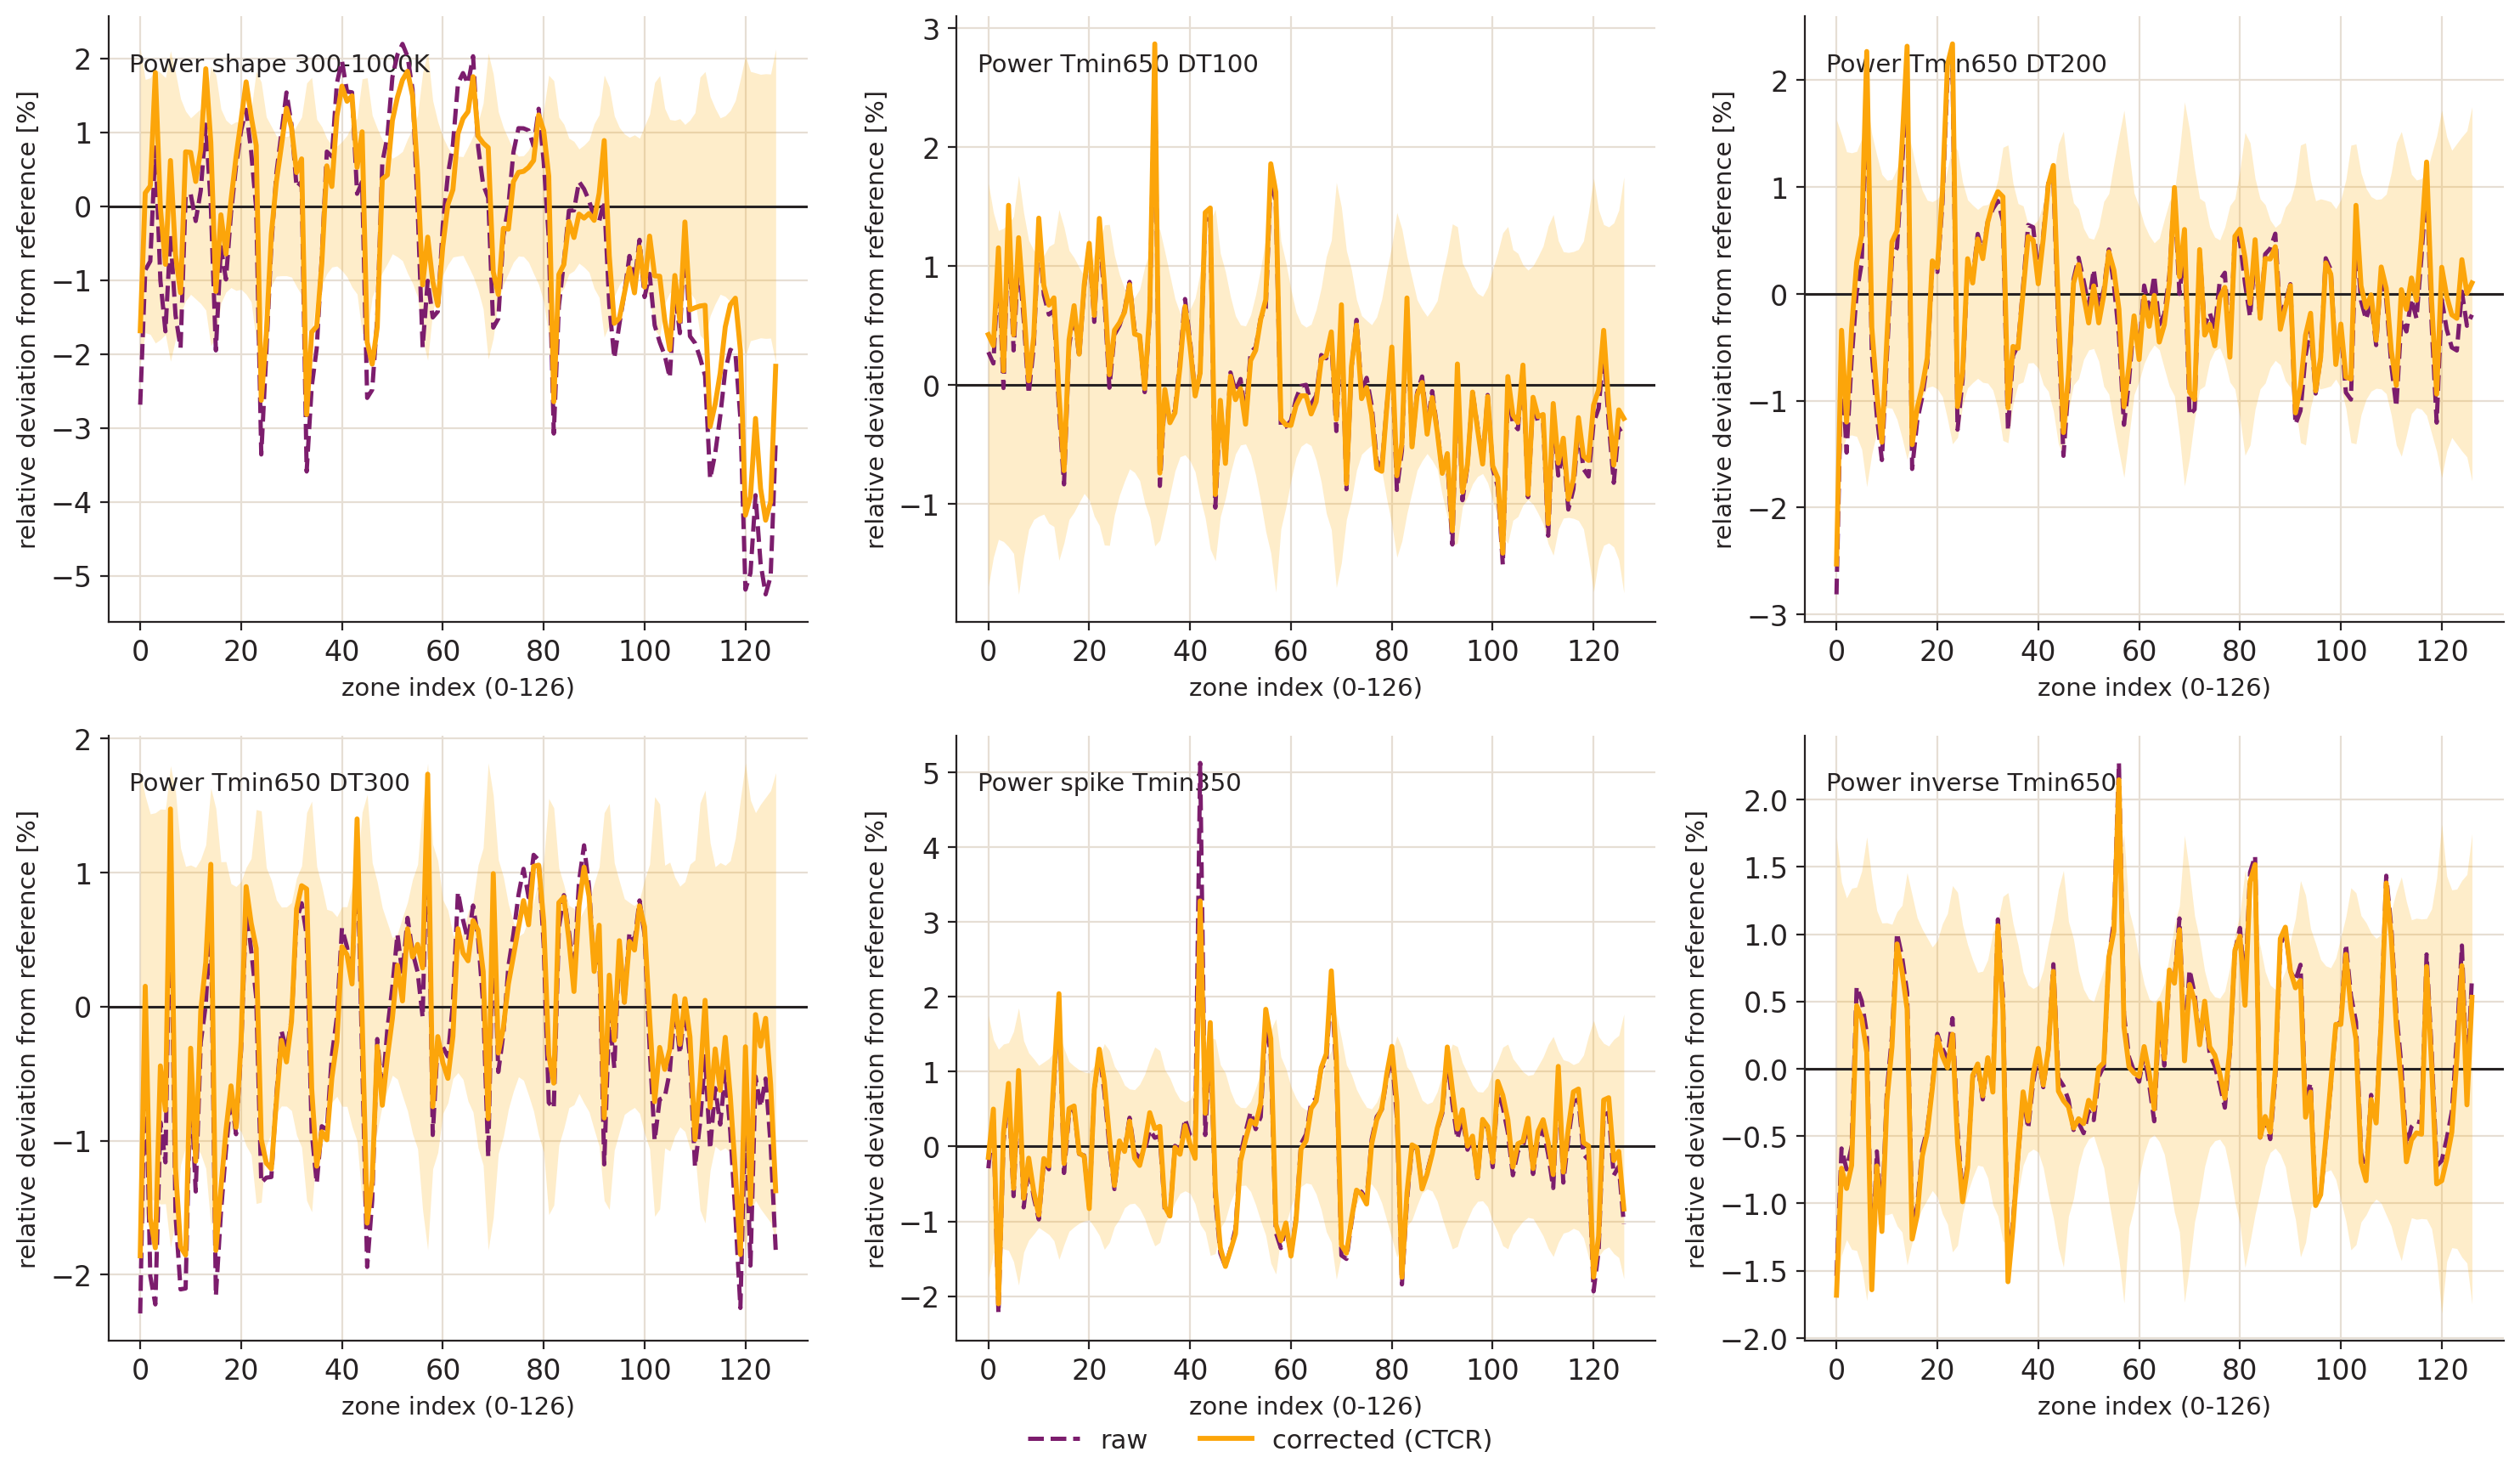
\includegraphics[width=140mm]{figures/fig5b_fission_source.png}
%   \caption{As Fig.~\ref{fig:fig5}, Test Cases 7--12.}
%   \label{fig:fig5b}
% \end{figure}

\section{Conclusions}
\label{sec:conclusions}

The interpolated (and CTCR-corrected) fission matrix inherits statistical noise from the database it is built from, but --- unlike a direct MC calculation --- has no uncertainty of its own to read off from any single simulation output; it has to be constructed by resampling the database itself. Of the three cheap ways of doing so, a zero-replica analytical model, derived from the branching structure of the fission process under the explicit simplifying assumption that only same-column coefficients are correlated, reproduces a genuine $N=150$ brute-force reconstruction's $k_{\text{eff}}$ uncertainty at least as well as an approach that requires measuring a full correlation matrix, and both improve markedly on assuming no correlation at all; on the fission-source RMS specifically, the two correlated approaches perform comparably to each other and somewhat better than the analytical model, though all three remain within the same order of magnitude of brute force. Folding either uncertainty source into a single budget, the CTCR's point-estimate benefit --- a 24\% reduction in mean absolute $k_{\text{eff}}$ discrepancy and a 25\% reduction in fission-source RMS discrepancy --- persists once both noise sources are accounted for, and 58\% of the remaining case-by-case discrepancies are statistically consistent with this combined floor. Where they are not, the residual is plausibly a limitation of the interpolation scheme's finite temperature grid rather than of the fission-matrix noise model used to characterize it --- a distinction this budget makes possible, and a natural target for future refinement independent of any further statistical work on the covariance itself.

\section*{Acknowledgments}

The authors would like to acknowledge that the research activity of the PhD project is sponsored by the Italian funding plan ``Piano Nazionale Ripresa e Resilienza'' (PNRR) and by Westinghouse Electric Company to support the development of methods for advanced reactors. This work has been carried over during the author's internship period at Westinghouse Electric Company. The methodology developed is an extension of the studies previously made during the author's internship activity at Argonne National Laboratory under the supervision and support of Dr.\ Nicolas Stauff and his research team.

\pagebreak
\bibliographystyle{style/ans_js}
\bibliography{bibliography}

\end{document}
